\chapter{Framework Valutati}
    Il primo passo necessario nella valutazione di questi frame\-work è stato
    chiarire bene quali applicazioni, tra le tre tipologie descritte nel
    capitolo \ref{chap:sam}, fosse possibile realizzare con essi.
    Durante la fase di ricerca abbiamo
    notato una gran confusione nell'attribuire a ciascun frame\-work il tipo di
    applicazione che permetteva di realizzare. Spesso il fatto che
    l'applicazione venisse eseguita all'interno di una componente nativa veniva
    pubblicizzato come se il frame\-work fosse in grado di creare una completa
    applicazione nativa anziché ibrida; in altri casi
    veniva confuso il concetto di \crosscomp{} (vedi \ref{sec:nativapp}) con
    quello di
    applicazione ibrida; in altri ancora non veniva mostrata la separazione
    concettuale che vi è tra frame\-work utili per la sola costruzione della
    logica e dell'interfaccia grafica dell'applicazione, e frame\-work che
    permettono d'incapsulare il contenuto web in una componente nativa creando
    così un'applicazione ibrida.

    Abbiamo così classificato \tisdk{} come frame\-work per la
    realizzazione di applicazioni native; Phonegap/Cordova, Rho Mobile e Sencha
    Touch come quelli dediti alla creazione di applicazioni ibride; \jqm{},
    \kendomob{} e \phonejs{} utili per implementare complete
    applicazioni web, e per la logica e l'interfaccia grafica di applicazioni
    ibride.

    \section{Framework per Applicazioni Native}
        \subsection{Titanium Appcelerator}
        \label{sec:titanium}
            \tisdk{} è una piattaforma gratis e open \mbox{source} di sviluppo di
            applicazioni mobili che permette la creazione di applicazioni native
            \crossplat{} per iOS, Android, BlackBerry e Tizen usando il
            linguaggio \js{}. Oltre alle applicazioni mobili questo frame\-work
            può essere utilizzato per creare applicazioni web.

            Titanium agisce come un ponte tra i sistemi operativi nativi e il
            codice dell'applicazione. La figura \ref{fig:ti_stack} illustra
            questa architettura.
            \begin{figure}[h]
                \centering
                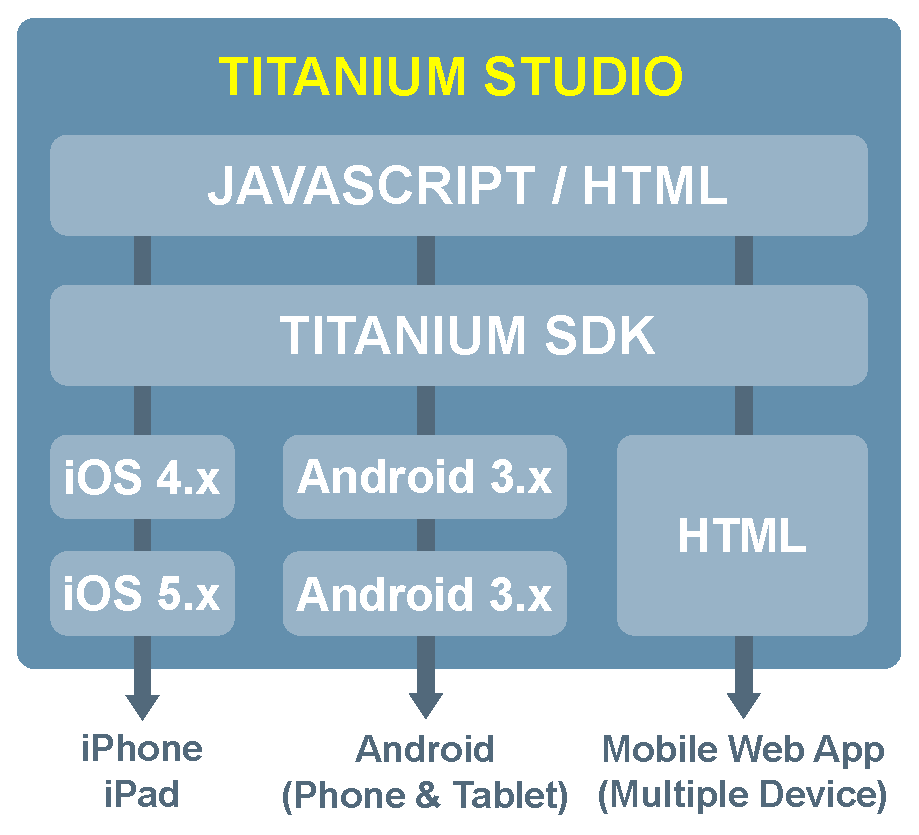
\includegraphics[keepaspectratio=true, width=12cm]{titanium-stack.eps}
                \caption{
                    Architettura nello sviluppo di un applicazione \crossplat{}
                    mediante Titanium Studio.
                }
                \label{fig:ti_stack}
            \end{figure}
            In fondo alla pila si trova il sistema
            operativo di destinazione: Android, iOS o il browser (per quanto
            riguarda le applicazioni web); sulla cima troviamo il codice
            dell'applicazione scritta in \js{} e in mezzo trova posto
            Titanium SDK insieme alle proprie API. Utilizzando tali interfacce
            nella propria applicazione è possibile fare azioni come mostrare la
            fotocamera, aprire nuove finestre, disegnare pulsanti, ecc.

            Titanium è descritto come un frame\-work \crosscomp{}\citep{Web:peptechlearn.blogspot.it} anche se l'uso che si fa di
            questo appellativo in questo caso non è del tutto corretto. Come
            spiega lo stesso amministratore delegato di Appcelerator Inc., Jeff
            Haynie, in un intervento online su
            \mbox{stackoverflow.com}\footnote{In quell'occasione era stato
            chiesto proprio come Titanium potesse funzionare riguardo alla
            creazione del codice nativo.\\L'intera discussione è consultabile
            all'indirizzo
            \url{http://stackoverflow.com/questions/2444001/how-does-appcelerator-titanium-mobile-work}}
            il modo di operare di Titanium è il seguente:
            \begin{quotation}
                \begin{hyphenrules}{english}
                Titanium takes your \js{} code, analyzes and preprocesses
                it and then pre-compiles it into a set of symbols that are
                resolved based on your applications uses of Titanium APIs. From
                this symbol hierarchy we can build a symbol dependency matrix
                that maps to the underlying Titanium library symbols to
                understand which APIs (and related dependencies, frameworks,
                etc) specifically your app needs. I'm using the word symbol in a
                semi-generic way since it's a little different based on the
                language. In iPhone, the symbol maps to a true C symbol that
                ultimately maps to a compiled .o file that has been compiled for
                ARM/i386 architectures. For Java, well, it's more or less a
                .class file, etc. Once the front end can understand your
                dependency matrix, we then invoke the SDK compiler (i.e. GCC for
                iPhone, Java for Android) to then compile your application into
                the final native binary.

                So, a simple way to think about it is that your JS code is
                compiled almost one to one into the representative symbols in
                nativeland. There's still an interpreter running in interpreted
                mode otherwise things like dynamic code wouldn't work. However,
                its much faster, much more compact and it's about as close to
                pure native mapping as you can get. [\ldots]
                \end{hyphenrules}
            \end{quotation}
            Ciò significa che il sistema fa tutto il possibile per creare codice
            nativo che rappresenti uno a uno quello che si è descritto in
            \js{} ma parte del nostro sorgente dovrà ancora essere
            interpretato a tempo di esecuzione. L'interprete \js{} viene
            inserito nel pacchetto in fase di compilazione e, a seconda della
            piattaforma di destinazione, sarà inserito
            \js{}Core\footnote{Maggiori dettagli e informazioni si possono
            trovare online all'indirizzo\\ \url{http://webkit.org/projects/javascript/}}
            per iOS o Rhino\footnote{Maggiori dettagli e informazioni si possono trovare
            online all'indirizzo\\ \url{https://developer.mozilla.org/it/docs/Rhino}}
            per Android e BlackBerry\citep{Web:KevinPost}.

            Visto che il codice \js{} viene ancora in parte interpretato,
            \crosscomp{} non è del tutto appropriato in quanto con tale
            aggettivo ci si riferisce ad una tecnica che permette, a partire da
            un certo sistema, di creare codice eseguibile per un secondo sistema
            avente caratteristiche e proprietà differenti da quello di
            partenza\citep{Web:Wiki.cross-compiling}.

            In ogni caso possiamo pensare di utilizzare il termine
            \crosscomp{} per indicare che Titanium, al termine del processo di
            compilazione, produce un pacchetto che per la
            maggior parte contiene codice nativo e specifico per una data
            piattaforma. Questa è una differenza sostanziale rispetto a quello
            che avviene nella compilazione di un'applicazione ibrida, dove nel
            pacchetto risultante è solo il codice della web view ad essere
            realizzato in codice nativo, mentre il codice sorgente web
            (\js{}, \html{} e \css{}) rimane intatto e viene poi interpretato
            completamente dal motore del browser a tempo di esecuzione.

            Titanium richiede che sulla macchina usata per lo sviluppo vengano
            installati e configurati gli SDK nativi per le piattaforme di
            destinazione. In particolare per le applicazioni Android bisogna
            installare l'Android SDK, mentre serve Xcode per le applicazioni
            iOS. Questo perché dopo la prima fase di elaborazione dei sorgenti
            fatta dall'SDK di Titanium (descritta nell'intervento succitato)
            serve usare l'SDK nativo per creare il pacchetto finale da
            installare sul dispositivo.

            \clearpage
            \noindent Detto questo passiamo ad elencare cosa Titanium offre da
            una visione più ad alto livello\citep[Cap.2 - Titanium
            Mobile Overview]{Book:Ti}:
            \begin{itemize}
                \item Strumenti dello SDK Titanium
                \item APIs Mobile
                \item Titanium Studio
                \item Moduli
                \item Servizi cloud di Appcelerator
            \end{itemize}

            \paragraph{Strumenti dello SDK Titanium}
                Come strumenti per compilare l'applicazione in un pacchetto
                installabile contenente codice nativo, Titanium SDK utilizza un
                insieme di script Python e altri strumenti di supporto che
                lavoreranno insieme a quelli forniti dagli SDK per lo sviluppo
                nativo\footnote{Da qui la necessità di lavorare in un ambiente
                configurato con gli SDK nativi delle piattaforme per le quali si
                desidera realizzare l'applicazione}. Tutto questo è trasparente
                agli occhi di uno sviluppatore che può così concentrarsi solo
                nella realizzazione della propria applicazione.

            \paragraph{APIs Mobili}
                Titanium fornisce un ricco insieme di API \js{} che danno
                accesso a centinaia tra componenti native per l'interfaccia
                utente e componenti non visuali. Queste API sono suddivise in
                vari insiemi come Titanium.UI (per quanto riguarda l'interfaccia
                utente) o Titanium.Network (per quanto riguarda il networking).

            \paragraph{Titanium Studio}
                Appcelerator mette anche a disposizione un proprio IDE gratuito
                per rendere più agevole lo sviluppo. Titanium Studio, appunto, è
                un ambiente di sviluppo integrato derivato da Eclipse, uno degli
                IDE open \mbox{source} più utilizzati. Con Titanium Studio è possibile
                scrivere, fare testing e debugging delle proprie applicazioni;
                inoltre sono presenti anche vari templates e applicazioni di
                esempio per rendere più semplice cominciare a creare
                applicazioni con Titanium SDK. Titanium Studio è stato
                pensato per essere l'unico software di cui si ha bisogno (oltre
                agli SDK nativi delle diverse piattaforme) per
                sviluppare con Titanium SDK; per questo motivo dal suo interno
                si ha la possibilità di installare e configurare l'SDK (al primo
                avvio) e successivamente eseguire aggiornamenti. In più è
                integrata la funzionalità che permette di scaricare nuovi moduli
                per estendere l'insieme delle APIs.

                L'uso di questo strumento non è obbligatorio, Titanium SDK
                ha una propria interfaccia a linea di comando che permette di
                gestire ogni aspetto dello sviluppo: inizializzare un
                nuovo progetto, compilarlo, eseguirlo. Inoltre questa
                interfaccia permette anche di
                installare e configurare l'SDK stesso.
                Ovviamente se si rinuncia a Titanium Studio non è garantito che
                in altri IDE si riescano a trovare i medesimi tool per il
                debugging.

            \paragraph{Moduli}
                Titanium è composto da una serie di moduli che estendono alcune
                funzioni principali delle API. Se si controlla la documentazione
                relativa si può trovare una lista di moduli base che estendono
                il nucleo del sistema e, inoltre, Appcelerator pubblica
                campioni di moduli gratuiti sul proprio repository git su
                \mbox{github.com}\footnote{Il repository ufficiale di tutti i
                moduli pubblicati è raggiungibile all'indirizzo\\
                \url{https://github.com/appcelerator/titanium_modules}}.
                Ovviamente ogni sviluppatore è libero di creare e distribuire
                gratuitamente o vendere i proprio moduli attraverso il
                Marketplace\footnote{Appcelerator Marketplace\\
                \url{https://marketplace.appcelerator.com/}}
                di Appcelerator. Titanium SDK supporta l'impiego dei moduli
                anche nello sviluppo delle applicazioni web, in questo caso la
                loro realizzazione consiste nello scrivere un puro modulo
                \js{} e non qualcosa scritto in Java o Objective-C.

            \clearpage
            \paragraph{Servizi cloud di Appcelerator}
                Appcelerator fornisce svariati servizi ACS (Appcelerator Cloud
                Services) che sono inclusi nella lista delle varie componenti
                fruibili attraverso le API. Alcune delle funzionalità offerte da
                questi servizi sono:
                \begin{itemize}
                    \item Invio di notifiche push
                    \item Gestione dell'utente
                    \item Salvataggio e manipolazione di foto
                    \item Integrazioni con i social network
                    \item Memorizzazione di file
                    \item Chat
                    \item Memorizzazione di dati in formato chiave-valore
                \end{itemize}
                Per poter usufruire dei servizi ACS nella propria applicazione,
                otre che ad utilizzare le relative API fornite è necessario
                registrare la propria app online sul sistema di gestione dei
                servizi ACS di Appcelerator.

            \subsubsection{Titanium SDK e il paradigma MVC}
            \label{subsub:alloy}
                Appcelerator fornisce il frame\-work Alloy che consente agli
                sviluppatori di strutturare le loro applicazioni secondo
                paradigma MVC (Model-View-Controller)\footnote{Per approfondire
                si può consultare l'indirizzo\\
                \url{http://en.wikipedia.org/wiki/Model-view-controller}}. Con
                questo frame\-work l'interfaccia viene costruita combinando file
                sorgenti scritti con i linguaggi XML e TSS (una versione personalizzata
                di \css{}) mentre il codice che
                riguarda la logica dell'applicazione è ancora \js{}.
                L'uso di Alloy necessita di un passaggio in più durante il
                processo di compilazione: i vari file sorgenti di
                un'applicazione Alloy vengono ``pre-compilati'' per generare
                tradizionali sorgenti \js{} di un'applicazione Titanium.

                In fase di inizializzazione di un nuovo progetto, Titanium Studio
                permette di impiegare o meno Alloy nello sviluppare
                l'applicazione; in ogni caso il processo di compilazione è, come
                già detto, completamente gestito da Titanium SDK e rimane
                invisibile allo sviluppatore.

    \section{Framework per Applicazioni Web}
    \label{sec:frameworkwebapp}

        Come descritto più volte questi frame\-work hanno una duplice funzionalità.
        Ognuno di essi può essere utilizzato indipendentemente per realizzare
        applicazioni web (\hyperref[sec:webapp]{vedi~\ref{sec:webapp}}), oppure
        può essere combinato ai frame\-work descritti nella
        sezione\hyperref[sec:frameworkhybrid]{~\ref{sec:frameworkhybrid}} per
        realizzare un'applicazione ibrida più soddisfacente.

        \subsection{JQuery Mobile}
        \label{subsec:jQuery}
            \jqm{} è un frame\-work per lo sviluppo di applicazioni mobili
            web che sono accessibili da tutti i dispositivi: smartphone, tablet
            e computer desktop. Esso è stato costruito sopra i robusti frame\-work
            \jq{} e \jq{} UI, che erano stati sviluppati per potenziare e
            agevolare la creazione dei tradizionali siti web.

            Per usare \jqm{} è sufficiente scaricare dal sito del
            produttore\footnote{\url{http://jquerymobile.com/download/}} il
            pacchetto in formato .zip contenente tutti i file \js{}, \css{} e
            PNG necessari\footnote{Dallo stesso sito c'è la possibilità di
            personalizzare il contenuto del pacchetto .zip in base alle proprie
            preferenze. Ad esempio è possibile alleggerire il pacchetto
            eliminando il supporto per le animazioni di transizione tra le
            pagine}. Una volta ottenuti, questi file vanno inclusi nella pagina
            \html{} che conterrà il codice della struttura dell'applicazione. A
            questo punto è sufficiente scrivere i normali tag \html{} decorati con
            particolari attributi \verb|data-*| per definire i vari componenti
            dell'interfaccia grafica dell'applicazione. Nel esempio \ref{cod:jquery}
            viene mostrata l'implementazione di un'applicazione composta da
            una sola schermata che al suo interno contiene un'intestazione con
            il titolo dell'applicazione e un semplice bottone con un icona a
            forma di ingranaggio.\clearpage
            \begin{lstlisting}[
                label={cod:jquery},
                caption={
                    Semplice applicazione jQuery Mobile. Da notare i riferimenti
                    aggiunti nell'intestazione del documento HTML necessari per
                    l'uso del frame\-work.
                }
            ]
  <!DOCTYPE html>
  <html>
    <head>
      <meta name="viewport" content="initial-scale=1,
        maximum-scale=1">
      <link
        rel="stylesheet"
        href="jquery.mobile-1.4.2.min.css" />
      <script src="jquery-1.9.1.min.js"></script>
      <script src="jquery.mobile-1.4.2.min.js"></script>
    </head>
    <body>
      <div data-role="page">
        <div data-role="header">
          <h1>jQuery Mob. App</h1>
        </div>
        <a data-icon="gear" class="ui-btn">Options</a>
      </div>
    </body>
  </html>
            \end{lstlisting}
            \jqm{} in fase di inizializzazione seleziona gli elementi in
            base ai loro attributi \verb|data-*| e li potenzia inserendo dei markup
            aggiuntivi aggiungendo nuove classi \css{} e applicando gestori per gli
            eventi. Questo permette allo sviluppatore di scrivere velocemente
            una pagina con una certa base semantica, sarà poi \jqm{} a
            dare all'applicazione una più complessa interfaccia utente. Se
            l'applicazione è composta da più schermate \jqm{} fornisce
            il concetto di pagina per poter modellare questi elementi, e
            implementa anche un sistema di navigazione \ajax{} (Asynchronous
            \js{} and XML) per supportare un ricco insieme di animazioni
            nella transizione tra le pagine. Per definire una pagina è
            sufficiente racchiuderne il contenuto in un tag \verb|<div>| con
            l'attributo personalizzato \verb|data-role="page"|. In uno stesso
            file \html{} possono essere inserite più pagine ma questo non è
            obbligatorio; è possibile usare file \html{} specifici per ogni pagina.
            Quando un utente che sta visualizzando una pagina naviga verso
            un'altra viene generato un evento catturato automaticamente dal
            sistema di navigazione \ajax{} che esegue una richiesta di caricamento
            per la nuova pagina. Se la pagina di destinazione è stata definita
            nello stesso file dove è presente la pagina di partenza si parla di
            navigazione interna, altrimenti si parla di navigazione esterna. Nel
            primo caso essendo già stato caricato il file \html{} entrambe le
            pagine sono presenti nel DOM\footnote{Document Object Model: è il
            modello a oggetti \js{} generato dal browser che rappresenta la
            struttura dell'attuale documento \html{} caricato.} e si avrà una
            veloce transizione animata dagli effetti forniti dal frame\-work;
            nel caso di navigazione esterna si dovrà attendere il caricamento
            del nuovo documento, durante il quale \jqm{} cerca gli
            elementi \html{} con l'attributo \verb|data-role="page"|, crea il
            relativo modello a oggetti e lo inserisce nell'attuale DOM. In
            entrambi i tipi di navigazione il DOM viene aggiornato con i
            contenuti relativi alla pagina da mostrare e non viene mai
            reinizializzato completamente. Questo comporta navigazioni più
            gradevoli alla vista dell'utente e il sistema di caricamento
            asincrono permette di visualizzare animazioni di caricamento in
            sovrapposizione alla pagina che si sta lasciando fino all'effettiva
            navigazione nella nuova pagina.

            \jqm{} mette a disposizione dello sviluppatore numerosi
            widgets (come bottoni, liste scorrevoli, switch, ecc...) per
            comporre l'interfaccia grafica. L'aspetto dell'applicazione può
            essere personalizzato utilizzando molti temi già forniti dal
            produttore; online è presente anche un tool per crearne di nuovi
            \footnote{ThemeRoller è reperibile all'indirizzo
            \url{http://themeroller.jquerymobile.com/}} ma non è fornita la
            funzionalità automatica di adattare l'aspetto a seconda della
            piattaforma sulla quale si sta eseguendo l'applicazione (vedi fig.
            \ref{fig:jquery}).

            Il frame\-work consente di essere esteso tramite l'aggiunta di nuovi
            plug-in e widgets personalizzati. Nuovi plug-in permettono di
            estendere le funzionalità del sistema mentre nuovi widgets
            consentono di arricchire l'interfaccia utente.
            \begin{figure}[h]
                \centering
                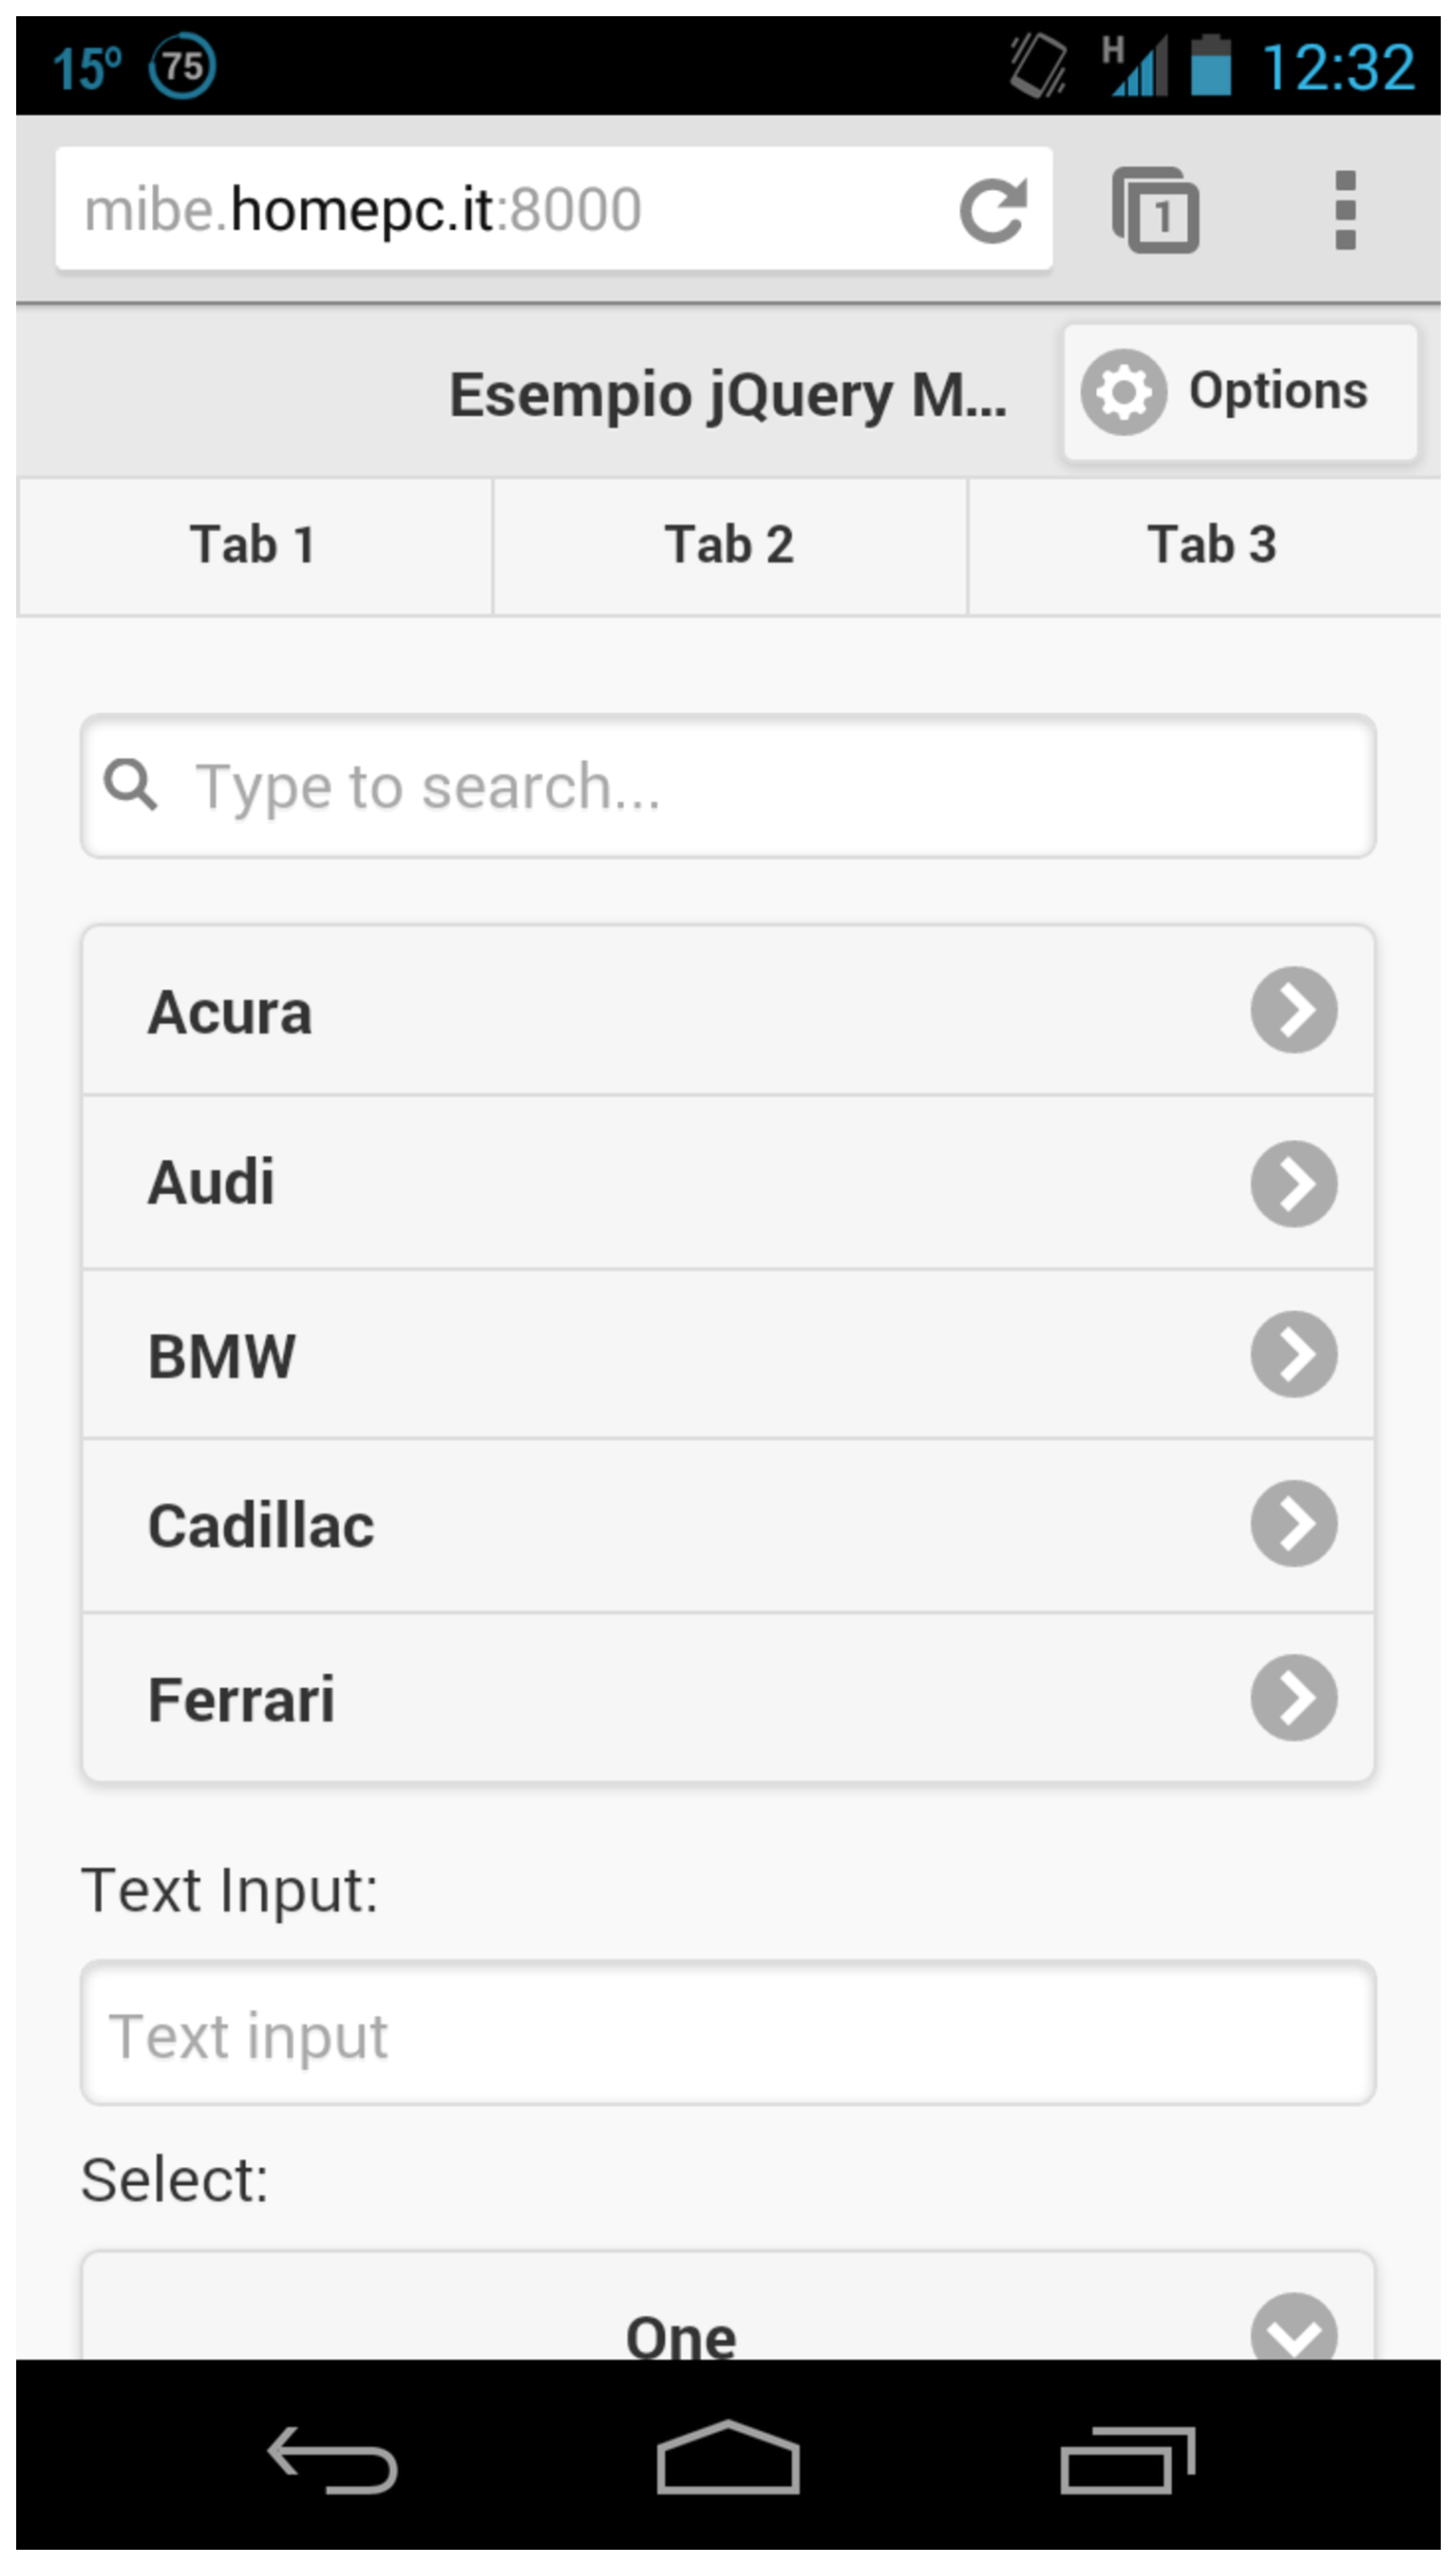
\includegraphics[keepaspectratio=true, width=0.32\textwidth]{jQuery-and}
                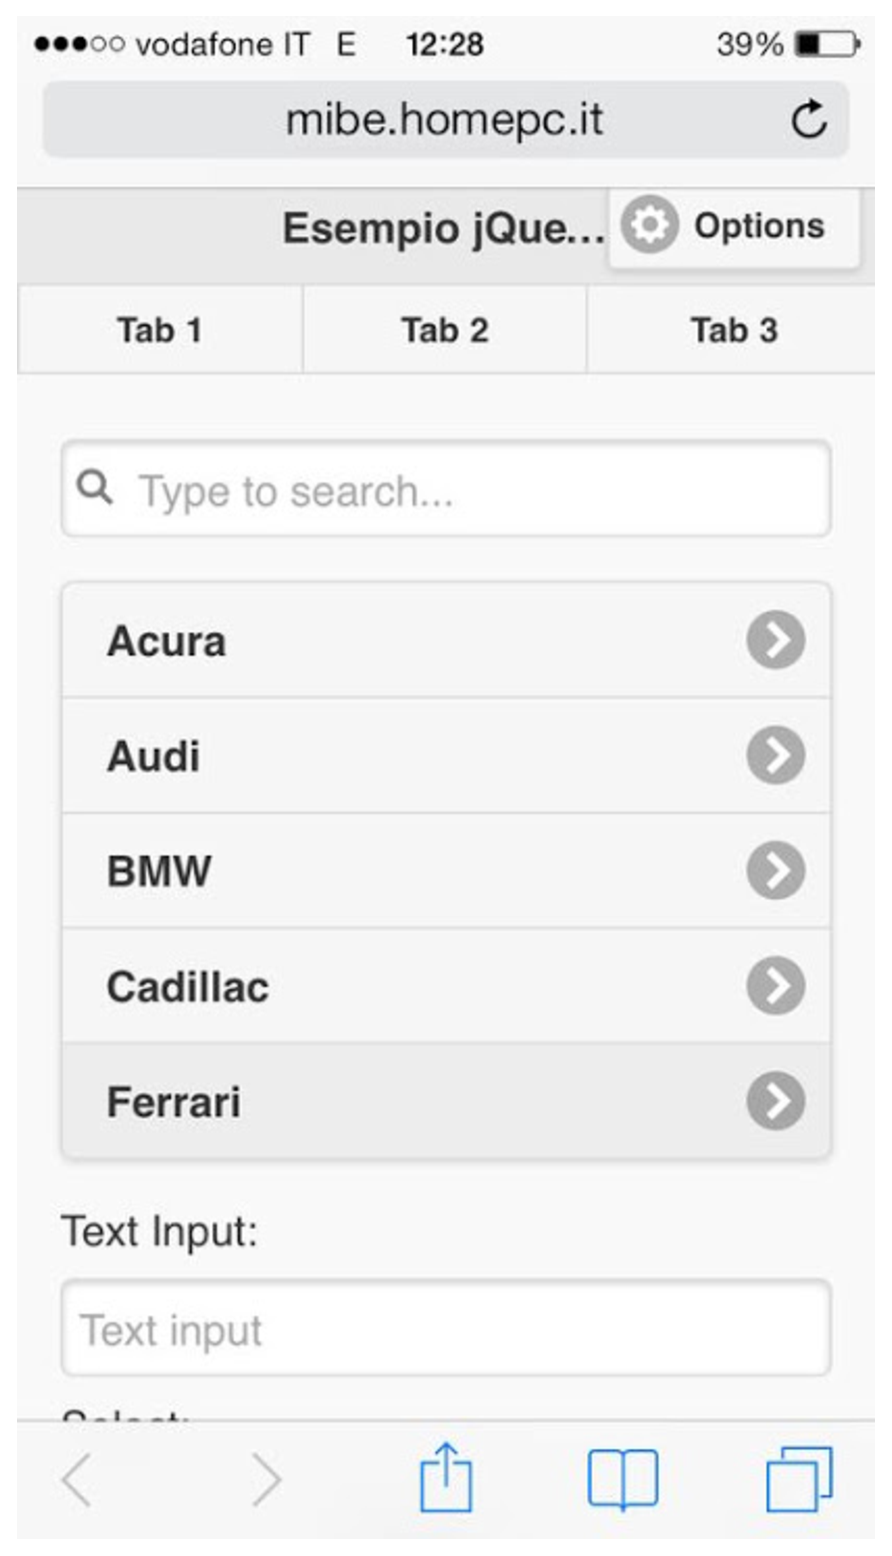
\includegraphics[keepaspectratio=true, width=0.32\textwidth]{jQuery-ios}
                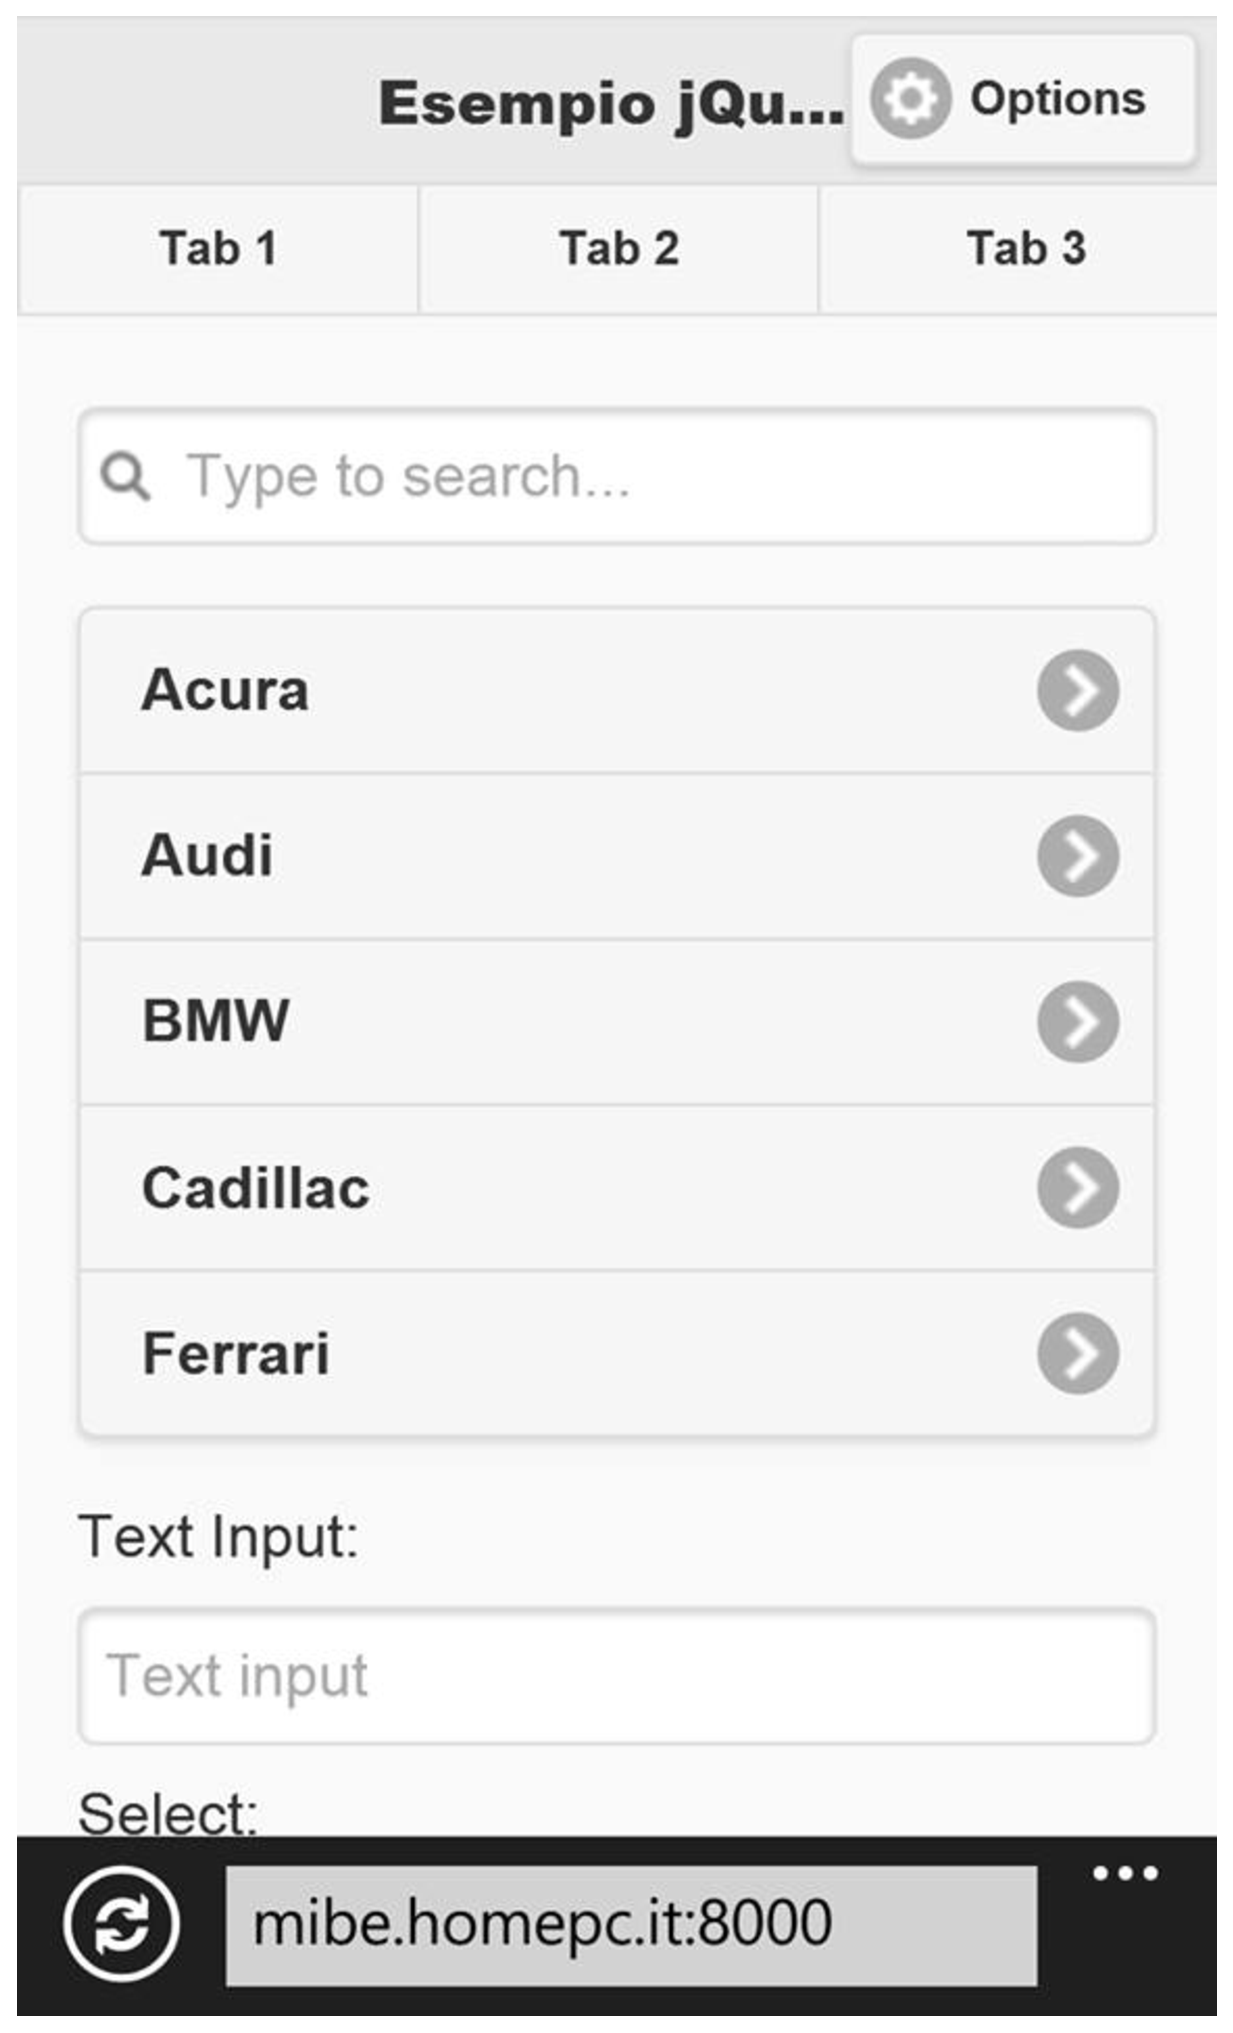
\includegraphics[keepaspectratio=true, width=0.32\textwidth]{jQuery-wp8}
                \caption{
                    Un esempio di applicazione web realizzata con \jqm{}.
                    Da sinistra a destra l'anteprima su piattaforma Android, iOS
                    e WindowsPhone8.
                }
                \label{fig:jquery}
            \end{figure}

        \subsection{KendoUI Mobile}
        \label{subsec:kendo}
            \kendomob{} è un frame\-work mobile completo che adatta
            automaticamente l'aspetto dell'applicazione alla piattaforma sulla
            quale è eseguita. Consiste di estensioni fondamentali per un
            frame\-work mobile come layouts, views, animazioni di transizione,
            e fornisce un ricco insieme di widgets per la costruzione
            dell'interfaccia grafica tra cui bottoni, liste, aree di input di
            testo e altro. Non è però solo per queste caratteristiche che viene
            definito un frame\-work completo, infatti \kendomob{} offre anche
            un utile componente per la gestione di sorgenti data, strumenti di
            validazione degli input, API per la globalizzazione e un frame\-work
            MVVM (Model View ViewModel). Come \jqm{}, \kendomob{} è
            basato sulla libreria \js{} \jq{}.

            \kendomob{} in versione di prova è scaricabile dal sito
            \url{http://www.telerik.com/download/kendo-ui-mobile}, quello che si
            ottiene è un pacchetto zip contenente tutti i file \js{} e \css{}
            necessari. La versione di prova può essere usata per apprendere
            l'uso del frame\-work ma non può essere usata per scopi commerciali
            quindi, a differenza di \jqm{}, è necessario    mettere in conto
            la spesa di acquisto della licenza se si intende commercializzare
            l'applicazione. I file \js{} e \css{} scaricati devono essere
            inseriti nel file \html{} che costituisce l'applicazione esattamente
            come è stato descritto per \jqm{}\footnote{Informazioni
            aggiuntive per iniziare a lavorare con \kendomob{} si possono
            trovare nel sito \url{http://docs.telerik.com/kendo-ui/getting-started/introduction}},
            inoltre, è necessario aggiungere uno script di inizializzazione che
            istruisce \kendomob{} su quale parte della pagina \html{} contiene il
            codice che implementa l'applicazione come mostrato nel frammento di
            codice \ref{cod:kendoinit}.
            \begin{lstlisting}[
                label={cod:kendoinit},
                caption={
                    Esempio di inizializzazione di un'applicazione KendoUI Mobile
                }
            ]
  <!DOCTYPE html>
  <html>
    <head>
      <link href="kendo.mobile.all.min.css"
        rel="stylesheet" />
      <script src="jquery.min.js"></script>
      <script src="kendo.mobile.min.js"></script>
    </head>
    <body>
      <div data-role="view" data-title="Home"> ... </div>
      <div data-role="view" data-title="Opzioni"> ... </div>
      ...
      <script>
        // Inizializza la nuova applicazione KendoUI Mobile
        var app = new kendo.mobile.Application(
          $(document.body)
        );
      </script>
    </body>
  </html>
            \end{lstlisting}
            Anche \kendomob{} sfrutta gli attributi \verb|data-*| per
            caratterizzare i vari tag \html{} dando loro un particolare aspetto
            grafico relativo al widget che si vuole definire; la stessa
            operazione può essere fatta direttamente da codice \js{}: nel
            frame\-work sono presenti le varie API per poter inizializzare ogni
            widget su un particolare elemento \html{}. Per esempio il frammento di
            codice \ref{cod:htmlbutton} mostra come definire direttamente in
            \html{} un pulsante \kendomob{} mentre nel listato \ref{cod:jsbutton}
            viene definito lo stesso widget ma tramite uno script \js{} che
            può essere anche inserito in un file separato.
            \begin{lstlisting}[
                label={cod:htmlbutton},
                caption={
                    Definizione di un bottone KendoUI Mobile in HTML tramite
                    attributo {\texttt{data-*}}.
                }
            ]
  ...
  <div id="foo" data-role="view">
    ...
    <a data-role="button">Click Me</a>
  </div>
            \end{lstlisting}
            \begin{lstlisting}[
                label={cod:jsbutton},
                caption={
                    Definizione di un bottone KendoUI Mobile in JavaScript
                    tramite l'uso delle apposite API.
                }
            ]
  ...
  <div id="foo" data-role="view">
    ...
    <a id="btnClickMe">Click Me</a>
  </div>
  <script>
    $("#btnClickMe").kendoMobileButton();
  </script>
            \end{lstlisting}

            Il punto di forza di \kendomob{} è la possibilità di creare
            applicazioni con aspetto nativo. Scrivendo codice una sola volta
            sarà infatti il frame\-work, all'avvio dell'applicazione, ad occuparsi
            di identificare la piattaforma e ad applicare il tema corretto. A
            prescindere da questa funzionalità è comunque possibile forzare
            l'utilizzo di uno stesso tema su piattaforme diverse. Attualmente
            \kendomob{} fornisce temi di aspetto nativo per le piattaforme
            Android, iOS, BlackBerry e Windows Phone 8 come mostrato in
            figura~\ref{fig:kendoui} ma, se si ha la necessità, è disponibile
            uno strumento online per la realizzazione dei propri temi
            personalizzati.
            \begin{figure}[h]
                \centering
                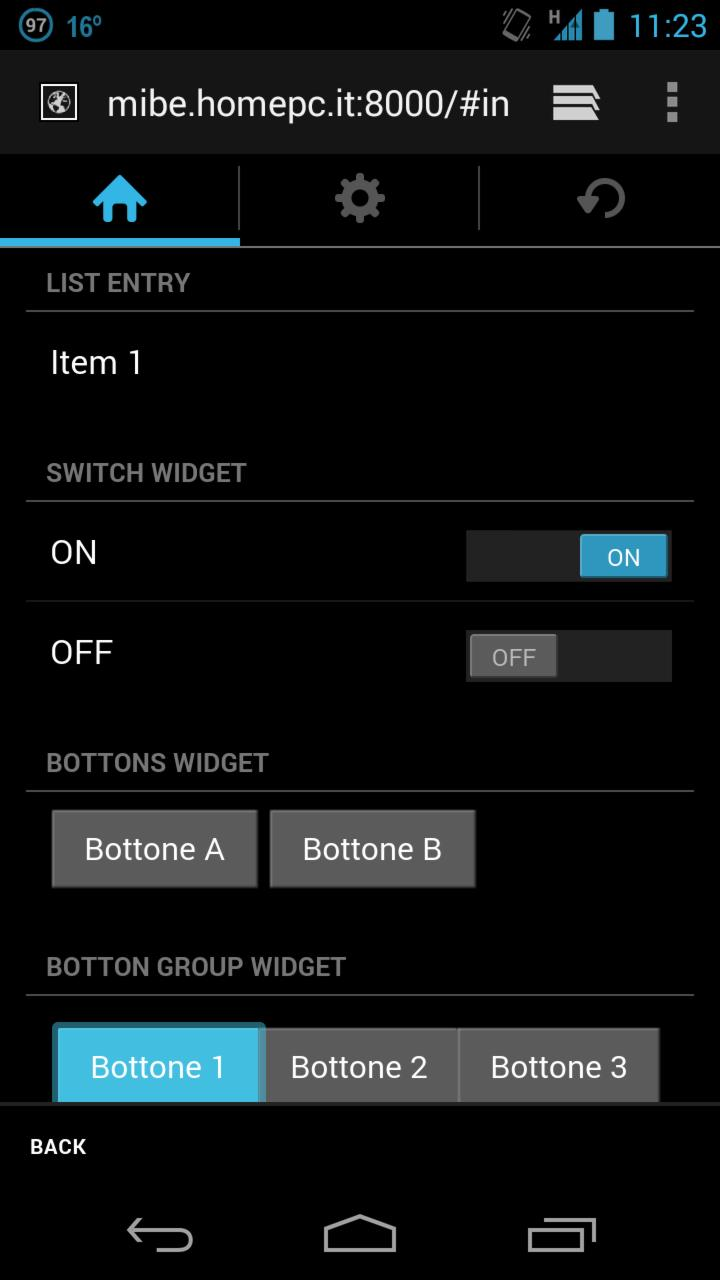
\includegraphics[keepaspectratio=true, width=0.32\textwidth]{kendoui-and}
                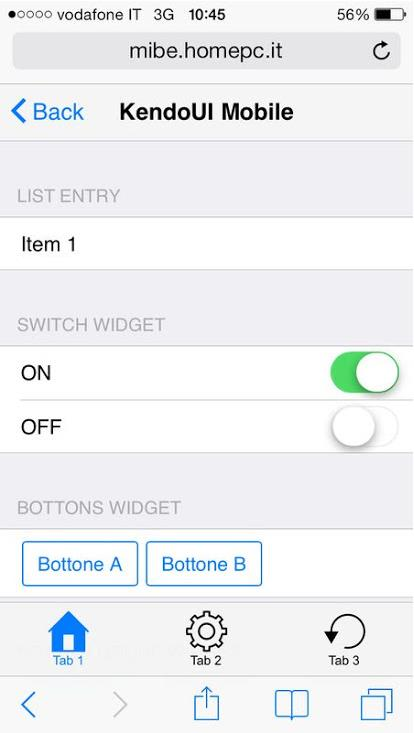
\includegraphics[keepaspectratio=true, width=0.32\textwidth]{kendoui-ios}
                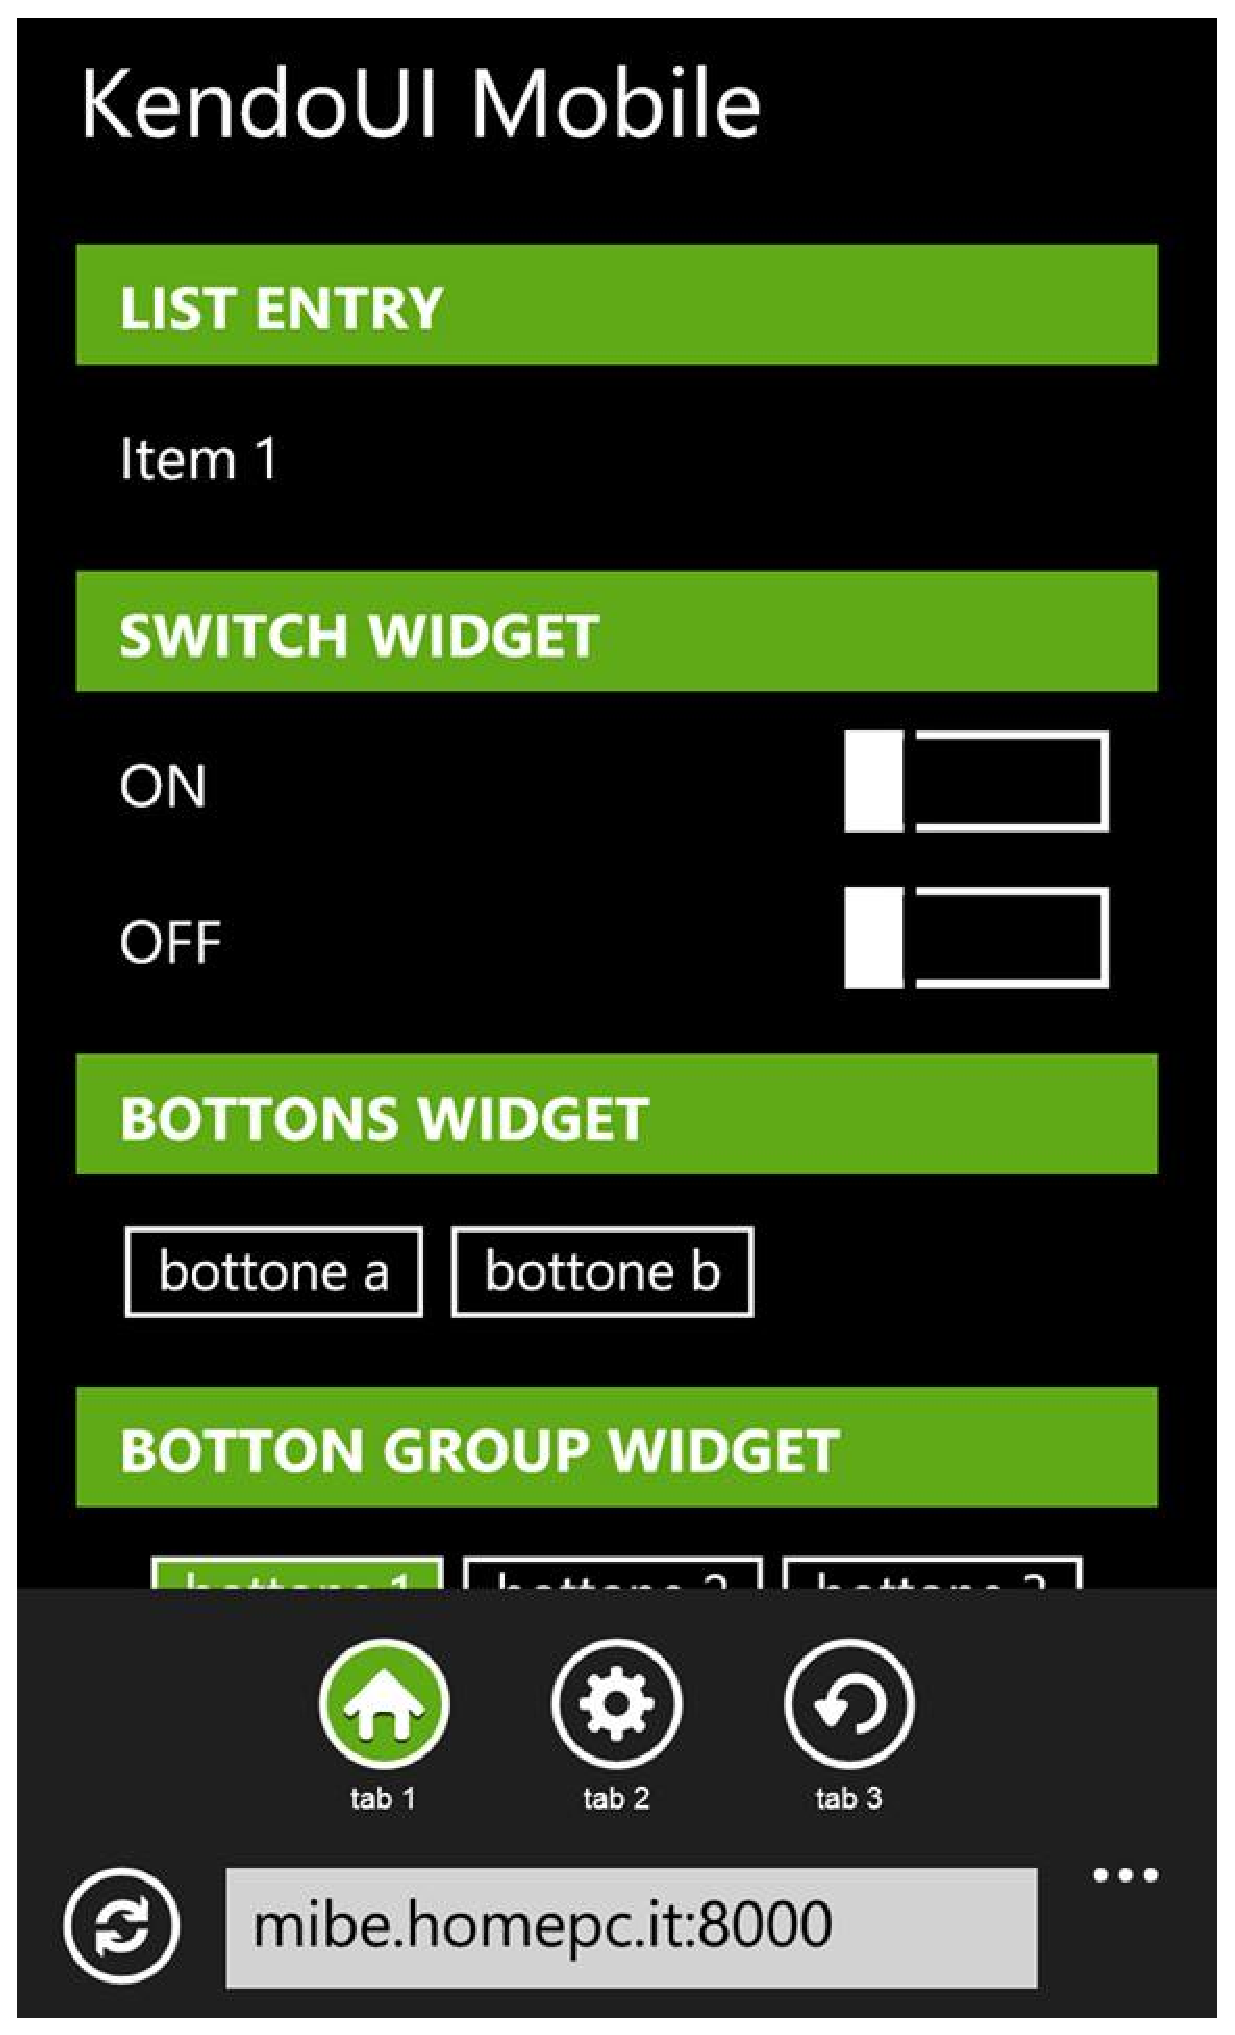
\includegraphics[keepaspectratio=true, width=0.32\textwidth]{kendoui-wp8}
                \caption{
                    Un esempio di applicazione web realizzata con \kendomob{}.
                    Da sinistra a destra l'anteprima su piattaforma Android, iOS
                    e WindowsPhone8.
                }
                \label{fig:kendoui}
            \end{figure}
            ThemeBuilder\footnote{Disponibile online sul sito web del produttore
            all'indirizzo \url{http://demos.telerik.com/kendo-ui/themebuilder/mobile.html}},
            con una semplice interfaccia grafica, consente di modificare colori e
            sfondi delle componenti grafiche dell'applicazione mostrando
            un'anteprima per ogni piattaforma supportata; una volta ottenuto il
            risultato desiderato è possibile esportare il tema in un file \css{} da
            utilizzare poi nella nostra app.

            Come precedentemente detto \kendomob{} non offre solo elementi
            di personalizzazione per l'interfaccia grafica. Il componente
            \mbox{DataSource} (KendoUI \mbox{DataSource}) è un'astrazione per la gestione e
            l'impiego di dati locali (array di oggetti \js{}) o remoti
            (XML, JSON, JSONP). Esso supporta completamente il CRUD (Create,
            Read, Update, Destroy) cioè fornisce le funzioni per creare,
            leggere, aggiornare e distruggere dati e consente sia alla parte
            locale che alla parte server di ordinare, impaginare, filtrare e
            raggruppare questi dati. Molti widgets di \kendomob{} supportano
            il data binding, cioè l'associazione dei dati agli elementi grafici;
            grazie a questo è possibile ad esempio mostrare in una lista i dati
            letti da un server o caricati localmente specificando non molto di
            più del formato con cui questi sono strutturati.

            Come detto poco fa \kendomob{} fornisce un frame\-work per lo
            sviluppo seguendo il paradigma MVVM; per provare a spiegare in cosa
            consiste tale modello ci serviamo di un esempio. Tipicamente in un
            qualsiasi genere di programma o applicazione è cosa comune dover
            manipolare certe entità; un'app che gestisce domande di laurea dovrà
            ragionevolmente trattare studenti, dove uno studente avrà
            particolari caratteristiche come nome, cognome e numero di matricola.
            Questo avrà due rappresentazioni: una in memoria mediante strutture
            dati opportune e un'altra grafica dove i dati dello studente saranno
            mostrati all'utente attraverso elementi grafici. L'utente può
            inoltre compiere determinate azioni su queste entità attraverso
            elementi grafici (es. sottoporre la domanda di laurea attraverso
            il tocco di un apposito tasto). Il paradigma Mo\-del-\-View-\-View\-Mo\-del
            formalizza le suddette rappresentazioni rispettivamente come Model e
            View, inoltre introduce il ViewModel, un terzo elemento che le mette
            in relazione, consentendo che le azioni e le modifiche fatte da
            parte dell'utente sulla View si ripercuotano sul relativo Model e
            viceversa. Impostare un'applicazione individuando queste parti
            porta alla scrittura di un codice più strutturato, più manutenibile
            nonché più leggibile.

            \kendomob{} fornisce un modo per internazionalizzare le pagine che
            compongono l'applicazione. Attraverso un particolare metodo offerto
            dalle API è possibile selezionare un particolare paese in modo da
            adottarne il formato di rappresentazione dei numeri, nomi dei mesi,
            di data e ora in maniera conforme agli standard locali.

            \html 5 ha introdotto gli attributi di validazione, questi particolari
            attributi hanno la capacità di forzare il browser ad avvisare
            l'utente che un certo elemento di input contenuto in un form debba
            essere compilato obbligatoriamente. KendoUI Validator offre un modo
            facile per gestire la validazione per gli elementi input di un form
            permettendo di personalizzare la gestione della validazione, ad
            esempio, accettando in input solo stringhe contenenti certe parole o
            numeri compresi in un dato intervallo.

            Come in \jqm{} è possibile realizzare un'intera applicazione
            composta da più schermate in una singola pagina \html{} attraverso l'uso
            del widgets view. Avendo la completa applicazione all'interno di un
            unico file si hanno ovvi vantaggi nella navigazione tra le sue schermate
            come già descritto per \jqm{}
            \hyperref[subsec:jQuery]{(vedi~\ref{subsec:jQuery})}.
            Per accelerare ulteriormente il caricamento delle views, se queste
            presentano la medesima struttura (per esempio sono composte da una
            intestazione contente una barra di navigazione e da un corpo),
            questa può essere definita in un particolare oggetto chiamato layout
            condiviso tra più views.

        \subsection{PhoneJS}
            PhoneJS è un frame\-work per realizzare applicazioni mobili
            single page application (SPA), che promette di fornire: un'
            esperienza utente ottimizzata per i dispositivi touch, elementi
            grafici (widgets) con
            aspetto nativo, agili strumenti di navigazione tra le schermate
            dell'applicazione, facile gestione delle schermate e un livello di
            accesso ai dati.

            La libreria PhoneJS sfrutta completamente jQuery e opzionalmente
            supporta KnockoutJS, per sviluppare l'applicazione attraverso il paradigma
            MVVM \hyperref[subsec:kendo]{(vedi~\ref{subsec:kendo})}.
            L'obiettivo è sempre quello di realizzare un'applicazione web cross-platform
            riusando completamente il codice.

            Come \kendomob{}, questo frame\-work è in grado di fornire all'applicazione
            un aspetto differente a seconda del dispositivo senza scrivere codice aggiuntivo.
            PhoneJS, infatti, identifica la piattaforma a tempo di esecuzione
            e applica automaticamente
            lo stile "nativo" appropriato a tutti i widgets e a tutti gli elementi
            di navigazione (vedi fig. \ref{fig:phonejs}).

            \begin{figure}[h]
                \centering
                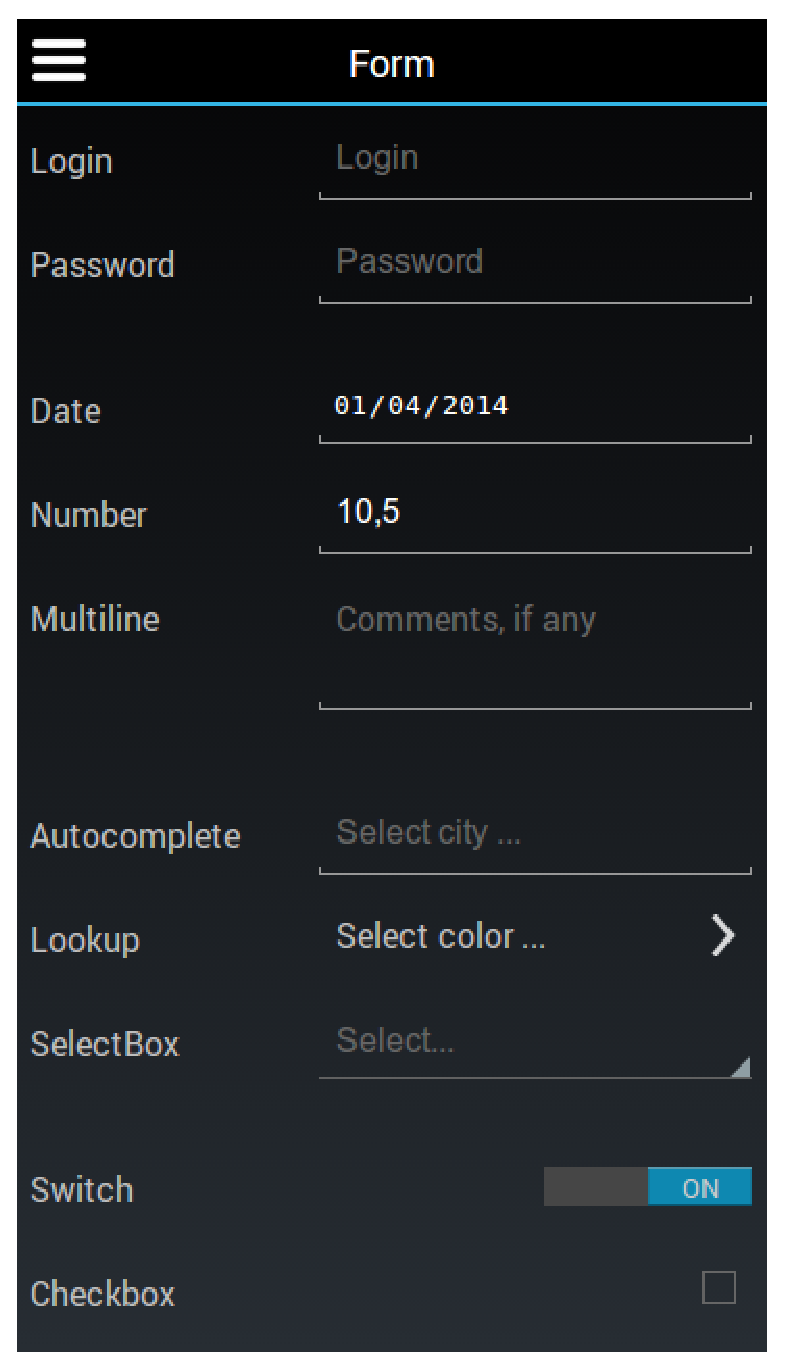
\includegraphics[keepaspectratio=true,
                width=0.32\textwidth]{phonejs-AND}
                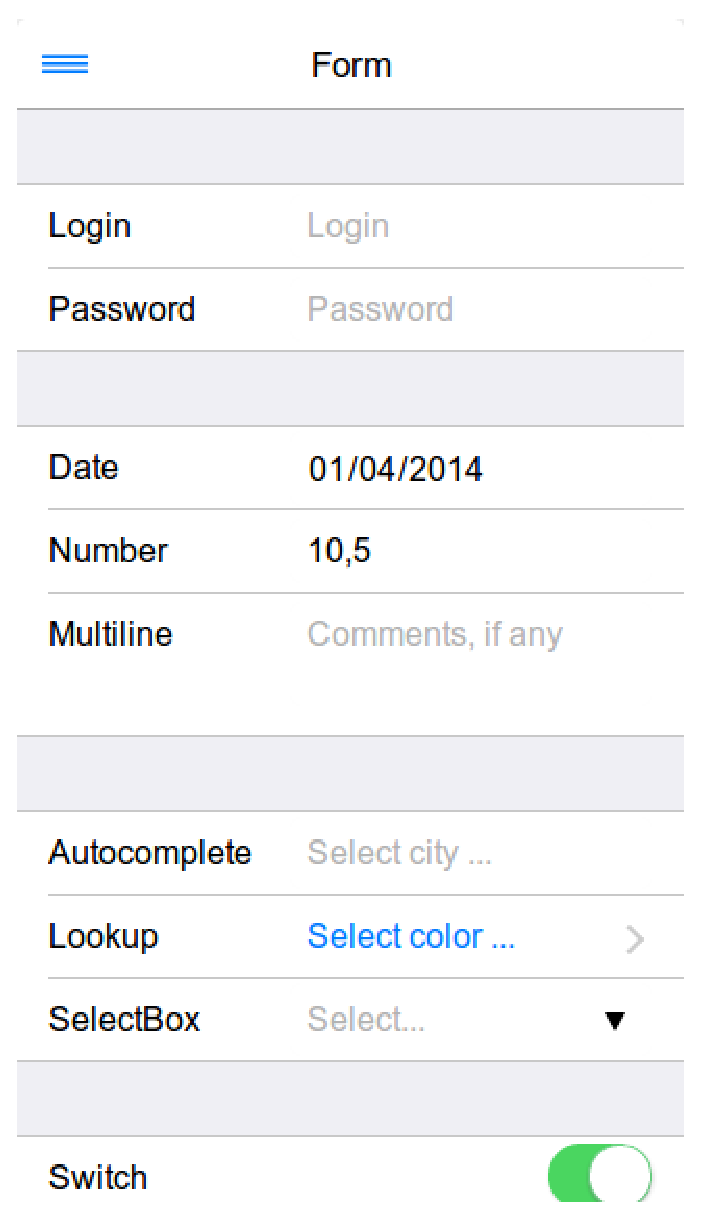
\includegraphics[keepaspectratio=true,
                width=0.32\textwidth]{phonejs-IOS}
                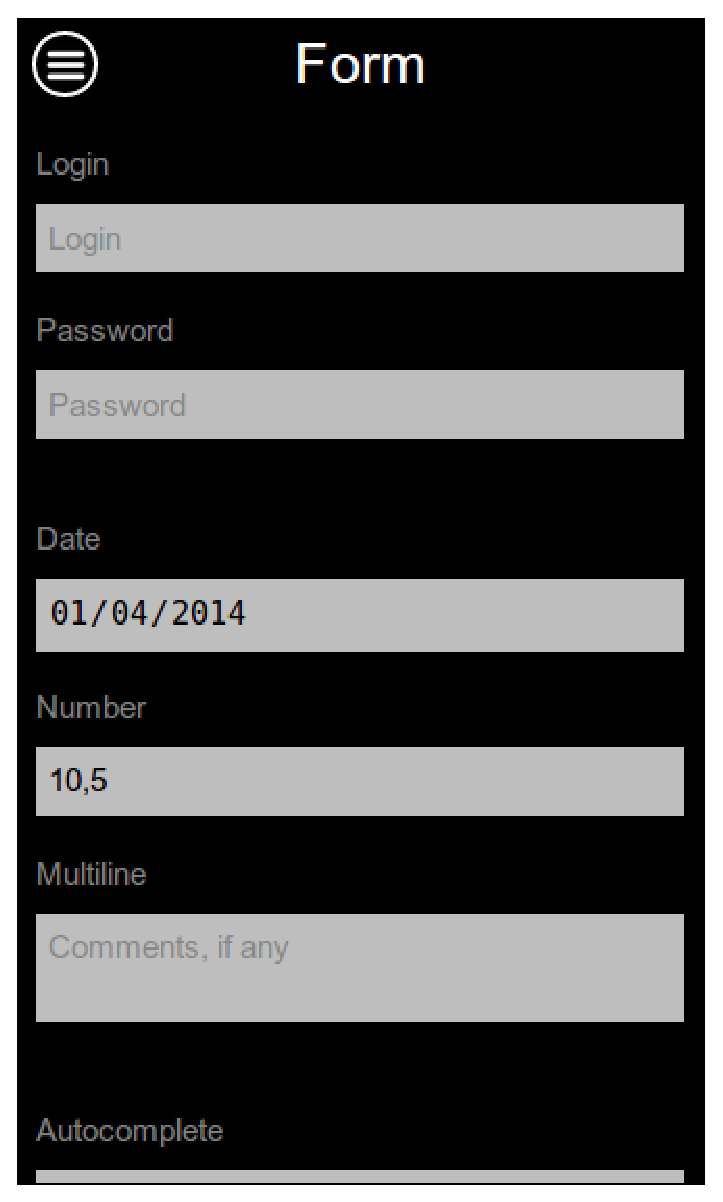
\includegraphics[keepaspectratio=true,
                width=0.32\textwidth]{phonejs-WIN}
                \caption{
                    Un esempio di applicazione web realizzata con PhoneJS.
                    Da sinistra a destra l'anteprima su piattaforma Android, iOS
                    e WindowsPhone8.
                }
                \label{fig:phonejs}
            \end{figure}

            PhoneJS include un vasto insieme di widget. Tipicamente,
            un widget è associato a dei dati e fornisce un'interazione con l'utente.
            Esso è rappresentato da un elemento HTML (contenitore), da un codice
            JavaScript per definirne il comportamento e da fogli di stile CSS
            per personalizzarne l'aspetto.
            Ogni widget può essere creato sfruttando jQuery oppure utilizzando
            KnockoutJS.

            PhoneJS fornisce tutti gli strumenti necessari per realizzare un'applicazione
            SPA: gestione e rendering delle schermate, navigazione attraverso url,
            layout specifico per il dispositivo, caching delle view e gestione degli stati.
            Il frame\-work usa le familiari regole di navigazione per definire la
            relazione tra l'URL nel quale l'utente naviga e la corrispondente schermata
            da caricare. Lo sviluppatore deve specificare la regola di navigazione e definire
            la schermata dell'applicazione, il frame\-work a run-time si occuperà di effettuare la
            navigazione.
            Quando si naviga in una view, questa sarà resa visibile attraverso un
            animazione di transizione, inoltre il frame\-work tiene traccia dell'avvenuta
            navigazione e aggiunge un bottone per tornare indietro. Questo comportamento
            di default può comunque essere cancellato.

            Per migliorare l'esperienza di sviluppo con PhoneJS è possibile usare
            il pacchetto DXTREME. Esso include le librerie PhoneJS e ChartJS e il
            supporto per Visual Studio 2012. Inoltre include un emulatore basato
            su browser che permette di fare debugging direttamente da Visual Studio.
            DXTREME non è gratis, ma è possibile usarne una versione di prova per
            30 giorni.

    \section{Framework per Applicazioni Ibride}
    \label{sec:frameworkhybrid}
        \subsection{Phonegap}
        \label{subsec:hybridpg}
            PhoneGap è un mobile development frame\-work prodotto da Nitobi, e
            acquistato da Adobe System il 4 ottobre 2011.
            Spesso ci si riferisce a PhoneGap col nome di Apache Cordova, ma è
            necessario fare una distinzione.
            Nel momento dell'acquisto della Nitobi da parte di Adobe, il codice
            di PhoneGap è stato donato all'Apache Software Foundation (ASF),
            questo per fare in modo che lo sviluppo del frame\-work godesse di
            tutti i benefici derivanti dalla licenza open \mbox{source}.
            Quello che avviene in sostanza è che sia le grandi compagnie, sia
            gli sviluppatori indipendenti contribuiscono a potenziare il codice
            di Apache Cordova che viene di fatto usato come incubatrice per PhoneGap.
            PhoneGap è diventato così una distribuzione di Apache Cordova\footnote{
            L'ipotesi più accreditata sulla scelta del nome Cordova
            è che quando il progetto PhoneGap è nato la Nitobi aveva gli uffici
            nella Cordova Street di Vancouver.}. All'inizio la differenza tra
            i due era solo nel nome, ma nel tempo PhoneGap ha reso disponibili
            strumenti addizionali per collegarsi ai servizi di Adobe, un esempio
            di questi è PhoneGap Build che verrà
            descritto successivamente. Le istruzioni per iniziare ad usare
            Apache Cordova e PhoneGap sono presenti rispettivamente su
            \url{https://cordova.apache.org/} e su
            \url{http://phonegap.com/}. Dal punto di vista dello sviluppatore di
            applicazioni mobili usare Apache Cordova o PhoneGap differisce solo
            per l'integrazione dei suddetti servizi, per il resto non ci sono
            differenze.

            Con PhoneGap come detto è possibile creare applicazioni ibride e quindi
            applicazioni in grado di sfruttare fotocamera, GPS, filesys\-tem e
            altri sensori del dispositivo. Per fare questo il frame\-work offre
            delle API JavaScript che combinate con un frame\-work UI come quelli descritti
            nel paragrafo\hyperref[sec:frameworkwebapp]{~\ref{sec:frameworkwebapp}}
            permettono di realizzare applicazioni mobili che sono distribuibili
            attraverso gli app store delle varie piattaforme sviluppando
            semplicemente con HTML5, CSS3 e JavaScript.

            Questo frame\-work fornisce inoltre un'interfaccia da riga di comando (CLI)
            che permette di usare i comandi per: creare l'applicazione, aggiungervi
            plugin, compilarla e installarla su un dispositivo o su un emulatore.
            Se si usa PhoneGap saranno inoltre disponibili comandi per eseguire
            la compilazione remota attraverso PhoneGap Build.

            Le APIs di PhoneGap sono consistenti tra le varie piattaforme mobili,
            l'applicazione può essere quindi portata su più dispositivi con
            sistemi operativi diversi attraverso piccoli accorgimenti, questa
            caratteristica rende quindi particolarmente semplice scrivere
            applicazioni mobili cross-platform.
            Attualmente PhoneGap è disponibile per le seguenti piattaforme:
            Amazon-Fireos, Android, Blackberry10, iOS, Windows Phone 7,
            Windows Phone 8, Tizen, Ubuntu \hyperref[fig:platformsupport]{(Vedi
            tab.~\ref{fig:platformsupport}).}
            {\footnotesize
                \begin{table}
                    \begin{tabularx}{\textwidth}{|l*{7}{|s}|}
                        \hline
                          & Android & Black\-Berry10 & iOS & WP7/8
                        & Tizen
                        \tabularnewline
                        \hline
                        PhoneGap CLI &\sprt{} Mac, Windows, Linux &
                        \sprt{} Mac, Windows & \sprt{} Mac & \sprt{} Windows & \notsprt{}
                        \tabularnewline
                        \hline
                        Plug-in Interface & \sprt{} & \sprt{} & \sprt{} & \sprt{} &
                        \notsprt{}
                        \tabularnewline
                        \hline
                        Accelerometer & \sprt{} & \sprt{} & \sprt{} & \sprt{} & \sprt{}
                        \tabularnewline
                        \hline
                        Camera & \sprt{} & \sprt{} & \sprt{} & \sprt{} & \sprt{}
                        \tabularnewline
                        \hline
                        Capture & \sprt{} & \sprt{} & \sprt{} & \sprt{} & \notsprt{}
                        \tabularnewline
                        \hline
                        Compass & \sprt{} & \sprt{} & \sprt{} (3GS+)& \sprt{} & \sprt{}
                        \tabularnewline
                        \hline
                        Connection & \sprt{} & \sprt{} & \sprt{} & \sprt{} & \sprt{}
                        \tabularnewline
                        \hline
                        Contacts & \sprt{} & \sprt{} & \sprt{} & \sprt{} & \notsprt{}
                        \tabularnewline
                        \hline
                        Device & \sprt{} & \sprt{} & \sprt{} & \sprt{} & \sprt{}
                        \tabularnewline
                        \hline
                        Events & \sprt{} & \sprt{} & \sprt{} & \sprt{} & \sprt{}
                        \tabularnewline
                        \hline
                        File & \sprt{} & \sprt{} & \sprt{} & \sprt{} & \notsprt{}
                        \tabularnewline
                        \hline
                        Geolocation & \sprt{} & \sprt{} & \sprt{} & \sprt{} & \sprt{}
                        \tabularnewline
                        \hline
                        Globalization & \sprt{} & \notsprt{} & \sprt{} & \sprt{} &
                        \notsprt{}
                        \tabularnewline
                        \hline
                        InAppBrowser & \sprt{} & \sprt{} & \sprt{} & \sprt{} & \notsprt{}
                        \tabularnewline
                        \hline
                        Media & \sprt{} & \sprt{} & \sprt{} & \sprt{} & \sprt{}
                        \tabularnewline
                        \hline
                        Notification & \sprt{} & \sprt{} & \sprt{} & \sprt{} & \sprt{}
                        \tabularnewline
                        \hline
                        Splashcreen & \sprt{} & \sprt{} & \sprt{} & \sprt{} & \notsprt{}
                        \tabularnewline
                        \hline
                        Storage & \sprt{} & \sprt{} & \sprt{} & \sprt{} localStorage
                        \& indexedDB & \notsprt{}
                        \tabularnewline
                        \hline
                    \end{tabularx}
                    \caption{Insieme degli strumenti e le
                    APIs disponibili per alcune delle piattaforme supportate.
                    La tabella completa è disponibile nella documentazione
                    di PhoneGap alla pagina \url{http://docs.phonegap.com/en/3.3.0/guide_support_index.md.html\#Platform\%20Support}}
                    \label{fig:platformsupport}
                \end{table}
            }

            E' interessante vedere come PhoneGap è riuscito a permettere la
            realizzazione di API JavaScript per accedere alle funzionalità
            dei dispositivi.
            Molti SDKs nativi forniscono una particolare componente chiamata
            Web View, all'interno della quale è possibile caricare del contenuto
            web che viene interpretato come se fosse stato aperto in
            un Browser.
            Inoltre il linguaggio nativo delle piattaforma offre la possibilità
            di usare, all'interno di queste Web View, codice JavaScript per
            eseguire codice nativo.
            Ad esempio su Android la Web View è realizzata con una classe Java
            che fornisce il metodo
    \begin{lstlisting}[language=MyJava]
  addJavascriptInterface(Object object, String name)
    \end{lstlisting}
            per permettere
            di scrivere codice JavaScript che attraverso la stringa name ha accesso
            ai metodi Java del parametro object.

            PhoneGap sfrutta tutto ciò per creare in fase di compilazione la
            cosiddetta shell, cioè una particolare
            Web View estesa con un livello che funge da ponte
            tra codice JavaScript e codice nativo, rendendo così possibile esporre
            agli sviluppatori dell'applicazione mobile un'interfaccia JavaScript
            che sfruttando il ponte sia in grado di invocare codice nativo.
            La shell rende la piattaforma PhoneGap estendibile tramite i cosiddetti
            plugins, cioè pacchetti creati per accedere al dispositivo e a quelle
            funzionalità che normalmente non sono disponibili per le applicazioni
            web. Un plugin è composto da un'interfaccia JavaScript che
            verrà usata per tutte le piattaforme, e da un'implementazione
            in codice nativo (ovviamente diversa per ogni piattaforma)
            della funzionalità offerta.
            E' importante notare che tutte le principali API di PhoneGap sono
            implementate come plugins.

            Descriviamo ora il processo di sviluppo da usare con PhoneGap.
            La prima cosa da fare è usare il CLI con il comando
    \begin{lstlisting}[language=MyBash]
  phonegap create "hello" "com.example.hello" "HelloWorld"
    \end{lstlisting}
            per creare l'applicazione di nome \verb|HelloWorld| all'interno della cartella
            \verb|hello|. Il parametro \verb|com.example.hello| serve per
            specificare l'identificatore univoco dell'applicazione.
            La cartella \verb|hello| conterrà la sottocartella \verb|www| dove
            vanno inserite le risorse necessarie al funzionamento dell'applicazione,
            quindi ci saranno: file HTML, CSS, JavaScript, immagini e il file
            \verb|config.xml| che contiene i metadati necessari per generare e
            distribuire l'applicazione.

            Per usare le API bisogna aggiungerle al progetto come plugin. Ad
            esempio per ottenere l'accesso alla fotocamera bisogna usare il comando
    \begin{lstlisting}[language=MyBash]
  phonegap local plugin add "org.apache.cordova.camera"
    \end{lstlisting}

            Dopo aver aggiunto tutti i plugin necessari l'applicazione può
            essere compilata e installata sul dispositivo (o su un emulatore).
            In questo caso è necessario specificare la piattaforma di destinazione,
            quindi se si vuole installare l'applicazione su Android il comando è
    \begin{lstlisting}[language=MyBash]
  phonegap run "android"
    \end{lstlisting}

            Il processo di compilazione di Phonegap come detto
            crea la shell nativa nella quale vengono interpretati i file HTML5, CSS3, e
            JavaScript che compongono l'applicazione. Il pacchetto
            risultante è un file che può essere distribuito attraverso gli stores
            delle varie piattaforme.

            Per creare il pacchetto nativo PhoneGap usa gli strumenti di compilazione
            degli SDKs nativi, è quindi necessario avere installato e configurato,
            sulla macchina
            usata per lo sviluppo, i Software Development Kits delle piattaforme
            di destinazione dell'applicazione.

            Per superare questa necessità Adobe ha creato un servizio chiamato
            PhoneGap Build\footnote{Il servizio è accessibile dal sito
            \url{https://build.phonegap.com}}.
            Inviando i file sorgenti al servizio, attraverso un
            pacchetto .zip o attraverso il repository GitHub, il processo di
            compilazione sarà eseguito direttamente da PhoneGap Build, permettendo
            poi di scaricare l'applicazione installabile sulle varie piattaforme.
            L'attuale versione di PhoneGap Build è la 3.3.0 ed è in grado di compilare
            applicazioni per iOS, Android e WindowsPhone 8. Per iOS serve comunque
            essere registrati tra gli sviluppatori Apple questo consentirà di
            testare le app su iPhone e iPad.
            Se si intende usare questo servizio bisogna cambiare il modo in cui
            vengono aggiunti i plugin: anziché usare il CLI occorre modificare
            il file \verb|config.xml|. Riferendosi sempre all'uso dell'API per
            l'accesso alla fotocamera, la riga da inserire nel file è la seguente
    \begin{lstlisting}[]
  <gap:plugin name="org.apache.cordova.camera"/>
    \end{lstlisting}

            Oltre alla possibilità di fare compilazione PhoneGap Build fornisce
            il cosiddetto Hydration, un'opzione di compilazione che se abilitata
            permette di testare le modifiche fatte all'applicazione senza doverla
            reinstallare sul dispositivo (attenzione non tutte le modifiche
            funzionano). Infine PhoneGap Build offre un server weinre per fare
            debugging in remoto, usando gli strumenti di debug tipici dello
            sviluppo web.

            Il processo di sviluppo con PhoneGap Build da una parte permette di
            poter iniziare a realizzare l'applicazione senza perder tempo a
            installare e configurare tutti gli SDKs nativi~\footnote{Si pensi
            che tecnicamente non è nemmeno necessario usare il comando
            phonegap create per inizializzare l'applicazione, ma semplicemente
            basta creare una cartella con tutti i file necessari, comprimerla
            in formato .zip e inviarla al servizio}, ma allo stesso tempo
            abbiamo notato che il servizio è molto lento, sia per il tempo speso
            ad inviare il codice sorgente e a scaricare il pacchetto, sia perché
            il processo di compilazione non sembra essere molto performante e
            spesso il sito mostra
            dei disservizi. Inoltre bisogna tener conto che non tutti i plugin
            esistenti per PhoneGap sono utilizzabili con il servizio
            PhoneGap Build, anche se la possibilità di aggiungere plugin di terze
            parti sta facendo crescere il numero di quelli disponibili.

            La principale forza di PhoneGap risiede nella sua semplicità.
            Il team di sviluppatori di PhoneGap ha intenzionalmente implementato
            solo il minimo comune denominatore delle APIs native. In questo modo
            è facile per PhoneGap supportare molte piattaforme. Potenzialmente
            una qualsiasi piattaforma che offre una web view può essere supportata
            da PhoneGap.

            La qualità dell'interfaccia utente in un'applicazione PhoneGap
            varia in base al frame\-work usato per realizzare la web app, e al
            motore di rendering delle pagine web della piattaforma.
            Il motore di rendering WebKit su iOS fornisce buone prestazioni, le
            Android Web View sono funzionali, ma hanno qualche notabile
            limitazione~\citep{Web:KevinSite}


        \subsection{RhoMobile Suite}
            \rhom{} Suite è un insieme di strumenti, librerie e servizi cloud
            offerti da Motorola Solution Inc. che consente lo sviluppo di
            applicazioni ibride. Ideato per creare applicazioni di uso aziendale,
            dove si utilizzano particolari dispositivi prodotti dalla stessa
            Motorola, è stato esteso per supportare anche piattaforme iOS
            (dalla versione 6.0 in poi), Android (dalla versione 2.3 in poi),
            Windows Mobile 6.x Professional, Windows Mobile 6.0 Standard,
            Windows CE 5, Windows CE 6, Windows CE 7 e Windows Phone 8.
            \rhom{} Suite è composto da RhoStudio, RhoMobile, RhoConnect,
            RhoHub e RhoGallery.
            \subsubsection{RhoStudio}
                RhoStudio è un potente plug-in per Eclipse che lo estende aggiungendo
                funzionalità per lo sviluppo, il debugging e il testing di
                applicazioni \rhom{}. È utilizzabile su PC, Windows e Mac e
                include RhoSimulator, uno strumento che consente di emulare
                vari dispositivi e piattaforme diverse per provare ad eseguire
                l'applicazione durante la fase del suo sviluppo.
            \subsubsection{RhoMobile}
                RhoMobile, analogamente alla shell offerta da \pg{}, è il contenitore
                nativo che consente all'applicazione mobile di essere installata ed
                eseguita sul dispositivo come se fosse nativa, sviluppandola
                comunque in codice \html{}, \css{}, \js{} e Ruby. In aggiunta
                alle funzionalità di questi linguaggi, \rhom{} fornisce
                frame\-work per l'accesso ai sistemi e ai dispositivi attraverso
                le sue librerie di API Rhodes e RhoElements.

                Rhodes è un insieme di API che consentono a tutte le applicazioni
                \rhom{} di accedere a funzionalità specifiche del dispositivo
                come fotocamera, localizzazione gps e uso del filesys\-tem attraverso
                due possibili interfacce: una in linguaggio Ruby e l'altra in
                \js{}. Rhodes è open \mbox{source} e gli sviluppatori possono
                contribuire al suo sviluppo.

                RhoElements è un insieme di API aggiuntive che ottimizza e personalizza
                l'accesso da parte di applicazioni \rhom{} a dispositivi
                Motorola Solution. Consente di accedere tramite interfacce
                sia \js{} che Ruby ad un particolare insieme di funzionalità
                come lettori di codici a barre e ad altre funzionalità
                hardware disponibili sono su questo genere di dispositivi
                aziendali.
            \subsubsection{RhoConnect}
                RhoConnect è un'applicazione server che può essere ospitata anche
                su un sistema privato e agisce come un ponte tra i dati presenti
                nel sistema e quelli presenti sui dispositivi mantenendoli sincronizzati.
                Con RhoConnect l'applicazione può gestire in maniera semplice
                simultaneamente più sorgenti dati.
            \subsubsection{RhoHub}
                RhoHub è un servizio di compilazione online offerto da Motorola
                per la creazione dei pacchetti nativi di applicazioni \rhom{}.
                Completamente integrato in RhoStudio da la possibilità di
                compilare le applicazioni senza avere la necessità di disporre
                localmente degli SDK nativi delle diverse piattaforme di
                destinazione.
            \subsubsection{RhoGallery}
                RhoGallery rende più semplice agli sviluppatori la distribuzione
                delle applicazioni. Una volta caricata l'applicazione nella
                galleria e inviato all'utente il relativo link, con un semplice
                click l'applicazione verrà installata automaticamente sul
                dispositivo. Inoltre, una volta caricato un nuovo aggiornamento,
                tutti gli utenti che utilizzano quell'applicazione riceveranno
                automaticamente un email di notifica.

                Diversamente dagli altri store online, RhoGallery è
                pensato per un uso aziendale permettendo di creare il proprio
                canale di distribuzione privato.


        \subsection{Sencha Touch}
            \senchat{} è un frame\-work per lo sviluppo \crossplat{} di
            applicazioni ad alte performance che impiega le medesime tecnologie
            della programmazione Web; le applicazioni prodotte sono
            impacchettate in file installabili proprio come quelle native ma
            sono implementate in codice \html{}5, \css{} e \js{}. Con \senchat{}
            si possono produrre applicazione per dispositivi Android, iOS,
            Windows Phone, Microsoft Surface Pro and RT e BlackBerry ma, essendo
            basato sulle tecnologie web, possono essere realizzate applicazioni
            riguardanti anche per questo settore.

            Il produttore distribuisce \senchat{} con due diverse licenze d'uso:
            una per uso commerciale e l'altra per lo sviluppo di progetti open
            \mbox{source}. In quest'ultimo caso è possibile scaricare il pacchetto
            software senza spese\footnote{Il download in licenza open \mbox{source} è
            disponibile all'indirizzo \url{http://www.sencha.com/products/touch/download/}.}
            ottenendo così il frame\-work completo.

            Oltre al frame\-work, il produttore fornisce \senchacmd{}\footnote{
            Questo strumento è scaricabile gratuitamente indipendentemente dalla
            licenza d'uso di \senchat{}. Il pacchetto d'installazione è
            disponibile all'indirizzo \url{http://www.sencha.com/products/sencha-cmd/download}},
            un'interfaccia utente a linea di comando indispensabile per la
            creazione, la configurazione e l'impacchettamento delle applicazioni.
            Tale strumento è disponibile per piattaforme Windows, Mac OS X, e Linux;
            una volta installato, con il semplice comando
            \begin{lstlisting}[language=MyBash]
  sencha generate app 'MyApp' './MyApp'
            \end{lstlisting}
            è possibile creare, per esempio, una nuova applicazione di nome
            \verb|MyApp| nella cartella \verb|./MyAppDir|.

            Di seguito elenchiamo il principale contenuto della cartella del
            progetto creato attraverso \senchacmd{}:
            \begin{description}
                \item[app/]\hfill \\
                    La cartella contenente i models, le views, i controllers e
                    gli stores dell'applicazione. Ognuno di questi elementi sono
                    definiti in file \js{} separati e suddivisi in specifiche
                    sottocartelle.
                \item[app.js]\hfill \\
                    File \js{} principale; il codice al suo interno definisce
                    l'applicazione indicando il suo nome, le icone utilizzate,
                    il codice da eseguire all'avvio e altri dettagli.
                \item[app.json]\hfill \\
                    Il file di configurazione dell'applicazione.
                \item[index.html]\hfill \\
                    Il file \html{} dell'applicazione
                \item[packager.json]\hfill \\
                    File di configurazione utilizzato da \senchacmd{} per creare
                    i pacchetti nativi dell'applicazione.
                \item[resurces/]\hfill \\
                    La cartella contenente i file \css{} e le immagini utilizzati
                    dall'applicazione.
            \end{description}
            A questo punto, una volta modificato il file \verb|packager.json| con
            le proprie preferenze è sufficiente dare il comando
            \begin{lstlisting}[language=MyBash]
  sencha app package build 'packager.json'
            \end{lstlisting}
            per creare il pacchetto per la piattaforma desiderata.

            Dalla struttura delle cartelle del progetto si evince che \senchat{} adotta
            l'architettura MVC nelle proprie applicazioni estesa con nuove componenti;
            questo approccio rende il codice più chiaro, testabile, facile da mantenere.
            Come mostrato in figura \ref{fig:sencha_mvc}, un applicazione è
            composta dunque da nuovi elementi introdotti in \senchat{} e da
            classici dell'architettura MVC:
            \begin{description}
                \item[Models]\hfill \\
                    rappresenta un tipo di dato nell'applicazione, per esempio un
                    applicazione di e-commerce avrà modelli per utenti, prodotti
                    e ordinazioni.
                \item[Views]\hfill \\
                    sono responsabili della visualizzazione dei dati da parte
                    degli utenti sfruttando le componenti di \senchat{}.
                \item[Controllers]\hfill \\
                    gestiscono le interazioni con l'applicazione ascoltando le
                    azioni intraprese dall'utente, come tocchi e swipe, ed eseguendo
                    il giusto codice.
                \item[Stores]\hfill \\
                    sono responsabili del caricamento dei dati all'interno
                    dell'applicazione alimentando componenti come List e DataView.
                \item[Profiles]\hfill \\
                    permettono di personalizzare facilmente l'interfaccia grafica
                    dell'applicazione per telefoni e tablet condividendo il più
                    codice possibile.
            \end{description}
            \begin{figure}[h]
                \centering
                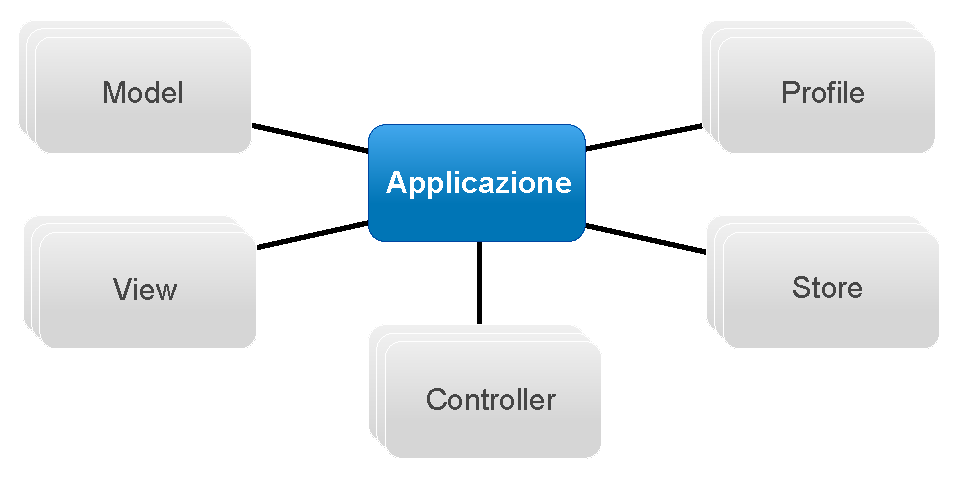
\includegraphics[keepaspectratio=true, width=\textwidth]{sencha-mvc}
                \caption{
                    Un applicazione \senchat{} è composta da Models, Views,
                    Controllers, Stores e Profiles
                }
                \label{fig:sencha_mvc}
            \end{figure}

            Come tutte le applicazioni ibride, anche quelle realizzate con
            \senchat{} hanno la possibilità di accedere a funzionalità proprie
            dei dispositivi (come utilizzare la fotocamera, ottenere la posizione
            dal GPS e avere accesso al filesys\-tem) tramite le opportune API
            della famiglia \verb|Ext.device.*|. A questo punto vale la pena
            spendere qualche parola in più per chiarire alcuni dettagli sul
            sistema di impacchettamento delle applicazioni. Per poter compilare
            l'applicazione in un pacchetto nativo installabile è necessario
            avere a disposizione gli SDK relativi alle piattaforme di destinazione.
            \senchacmd{}, una volta configurato, è in grado di creare pacchetti
            solo per piattaforme Android e iOS, ma dalla versione 2.3 è stato
            inserito il supporto per lavorare insieme a \pg{} e Cordova così da
            riuscire a supportare anche Windows Phone e BlackBerry. Un aspetto
            importante da sottolineare è che se si decide di lavorare con uno
            qualunque di questi frame\-work, l'uso delle API \verb|Ext.device.*| per
            l'accesso al dispositivo rimane ancora valido; sarà \senchacmd{} che
            durante il processo di compilazione si occuperà di utilizzare le
            relative API Cordova o \pg{} necessarie. Un altro aspetto da
            tenere in considerazione è il fatto che se si utilizza Cordova è
            ancora necessario lavorare insieme agli SDK di Windows Phone e BlackBerry
            che devo essere presenti in locale; se invece si utilizza \pg{} è
            possibile ovviare a questo inconveniente utilizzando il suo servizio
            di compilazione online \pgb{}. Qualunque soluzione si scelga di
            adottare, dopo aver creato un progetto, è sufficiente utilizzare
            ancora \senchacmd{} per abilitare il supporto di Cordova o \pg{} e,
            fatto questo, i comandi per la compilazione rimarranno gli stessi.

            \senchat{}, a differenza di altri della sua categoria, non è un
            frame\-work che offre solo la propria shell nativa per creare
            applicazioni ibride: tra le proprie APIs sono disponibili numerosi
            widgets per creare una consistente interfaccia grafica
            (vedi fig.~\ref{fig:senchaui}) così da non dover ricorrere a
            frame\-work aggiuntivi come nel caso di \pg{} e \rhom{}. Sono anche
            forniti numerosi temi con aspetto nativo per le piattaforme che
            supporta, e all'interno del file di configurazione dell'applicazione
            \verb|app.json| è possibile specificare quale tema utilizzare a
            seconda della piattaforma rilevata in fase di caricamento.
            \begin{figure}[h]
                \centering
                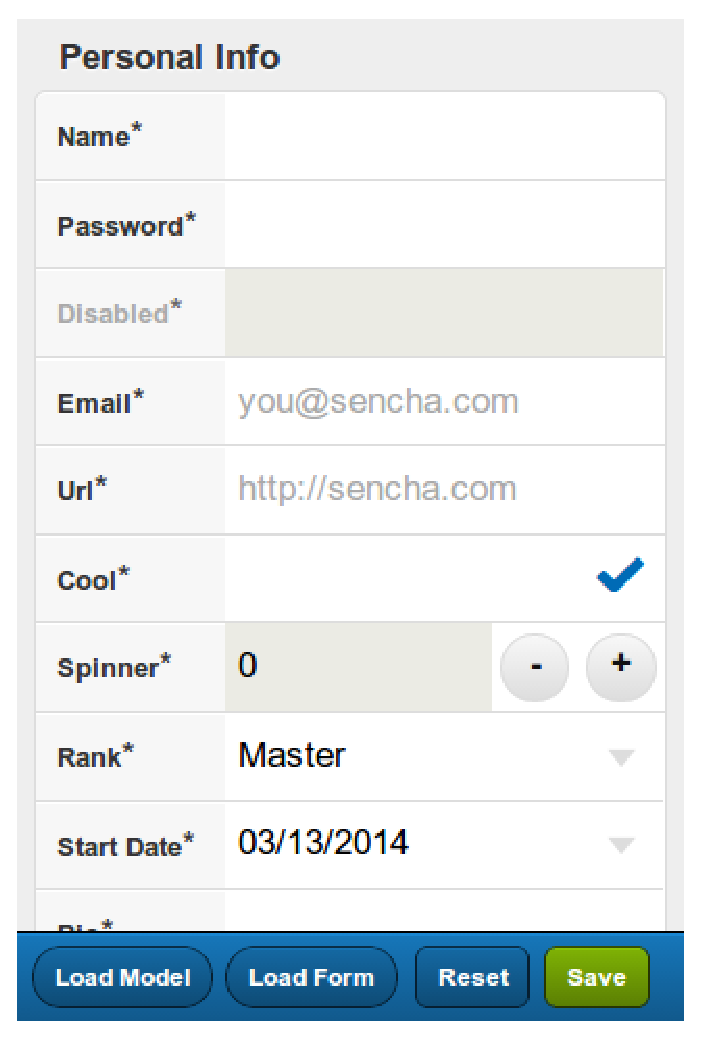
\includegraphics[keepaspectratio=true, width=0.45\textwidth]{sencha-ui-1}
                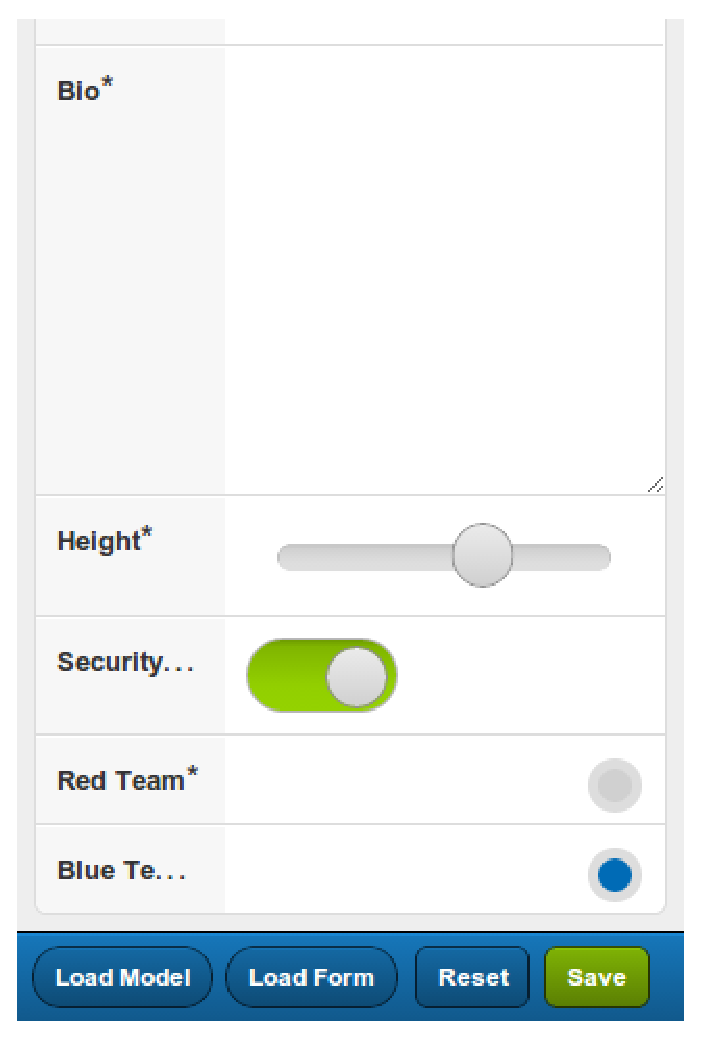
\includegraphics[keepaspectratio=true, width=0.45\textwidth]{sencha-ui-2}
                \caption{
                    Esempio di alcuni widget disponibili in \senchat{}.
                    Il tema grafico mostrato è quello generico del frame\-work e
                    non specifico per nessuna piattaforma.
                }
                \label{fig:senchaui}
            \end{figure}

    \section{Conclusioni}
        Classificare e valutare le funzionalità offerte da questi frame\-work
        ha permesso, a noi e al nostro tutore aziendale, di fare chiarezza su cosa
        li distinguesse realmente, così
        da poter decidere con quali di questi realizzare un'applicazione di prova utile
        per un'analisi più approfondita.
        La scelta naturale è stata quella di creare un'applicazione con due
        frame\-work che adottassero approcci diversi: sono stati quindi scelti
        \tisdk{} per la creazione di un'applicazione nativa, e
        PhoneGap per la realizzazione di quella ibrida.
        Il tutore ci ha lasciato libera scelta sul frame\-work per l'interfaccia
        grafica da usare assieme a PhoneGap. Colpiti dalla semplicità d'uso,
        dalla capacità di adattare l'aspetto a quello della piattaforma e
        dalle prestazioni osservate in applicazioni d'esempio, abbiamo deciso
        di utilizzare KendoUI Mobile.

